%%This is a very basic article template.
%%There is just one section and two subsections.
%\documentclass{llncs}
\documentclass[pldi,nocopyrightspace]{sigplanconf}
\usepackage{amsfonts}
\usepackage{rotating}
\usepackage{amsmath} 
\usepackage{multicol}
\usepackage{multirow}
\usepackage{courier}
\usepackage{listings}
\usepackage{natbib}
\usepackage{xspace}

\usepackage{qtree}

\usepackage{color}
\usepackage{pgfplots}

\usepackage{alltt}

%\usepackage{wrapfig}
%\usepackage[normalsections, normalmargins, normalindent,normaltitle]{savetrees}
\newtheorem{define}{Definition}
%\newtheorem{lemma}{Lemma} 
%\newtheorem{theorem}{Theorem} 
%\newtheorem{example}{Example}
   
   
\newcommand{\denot}[1]{\llbracket #1 \rrbracket}
\newcommand{\pred}{\phi}
\newcommand{\scond}{\scarg{\pred}} 
\newcommand{\scarg}[1]{\lfloor #1 \rfloor}
\newcommand{\ncond}{\ncarg{\pred}}
\newcommand{\ncarg}[1]{\lceil #1 \rceil}
\newcommand{\nc}{ \emph{NC}}
\newcommand{\sfc}{ \emph{SC}}
\newcommand{\true}{\emph{true}}
\newcommand{\false}{\emph{false}}
\newcommand{\code}[1]{$\tt  #1$\normalsize}
\newcommand{\smallcode}[1]{\scriptsize $\tt  #1$\normalsize}
\newcommand{\codet}[1]{\small {\tt  #1}\normalsize}
\newcommand{\mcode}[1]{\small {\tt  #1} \normalsize}
\newcommand{\integerop}{ \scriptsize \emph{\rm{\ intop \ }} \normalsize} 
\newcommand{\predop}{ \scriptsize \emph{\rm{\ predop \ }} \normalsize} 
\newcommand{\select}{\emph{select}}
\newcommand{\deref}{\emph{deref}}
\newcommand{\ap}{\pi}
\newcommand{\interval}{bracketing }
\newcommand{\Interval}{Bracketing }
\newcommand{\val}{\mathfrak{e}}
\newcommand{\alloc}{\emph{alloc}_\emph{id}}
\newcommand{\memap}{\ap_{\emph{mem}}}
\newcommand{\eval}{\emph{eval}}
\newcommand{\df}{\delta}
\newcommand{\assign}{\leftarrow}
\newcommand{\starstar}{*\hspace{-2.5pt}*}

\usepackage{wrapfig}
\usepackage{color}
\usepackage{comment}
\usepackage{newalg}
\usepackage{minibox}

\newcommand{\aenv}{\mathbb{E}}
\newcommand{\astore}{\mathbb{S}}
\newcommand{\kstore}{\astore_{K}}
\newcommand{\vstore}{\astore_{V}}
\newcommand{\sumenv}{\mathbb{G}}
\newcommand{\partenv}{\mathbb{A}}
\newcommand{\instenv}{\mathbb{I}}
\newcommand{\indexedloc}{\langle \alpha \rangle_i}
\newcommand{\cenv}{\mathbb{C}}
\newcommand{\newval}{\emph{newval}}
\newcommand{\abstractloc}{\delta}
\newcommand{\varalloc}[2]{\eta_{#1}\{#2\}}

\usepackage{amsthm}
\newtheorem{theorem}{Theorem}
\newtheorem{lemma}{Lemma}
\newtheorem{corollary}{Corollary}
%\newtheorem{proof}{Proof}
\theoremstyle{definition}
\newtheorem{definition}{Definition}



\newtheorem{example}{Example}
\newcommand{\summary}{\Delta}

\newcommand{\irule}[2]%
   {\mkern-2mu\displaystyle\frac{#1}{\vphantom{,}#2}\mkern-2mu} 
\newcommand{\irulelabel}[3]
{
\mkern-2mu
\begin{array}{ll}
\displaystyle\frac{#1}{\vphantom{,}#2} & #3
\end{array} 
\mkern-2mu
} 

\newcommand{\ds}{\delta}

\newcommand{\ra}{\rightarrow}

\newcommand{\lbrct}{{\rm [}}
 \newcommand{\rbrct}{{\rm ]}}
 \newcommand{\emptylist}{\lbrack \ \rbrack}
 \newcommand{\mylist}[1]{\lbrack #1 \rbrack}
 \newcommand{\todo}[1]{ {\color{red}{ TODO: #1}}}

\newcommand{\sys}{$\boldsymbol{\lambda^2}$\xspace}


\newcommand{\id}[1]{\mathit{#1}}

% \category{D.2.4}{Software Engineering}
% {Software/Program Verification}
% \terms
% Languages, Verification, Experimentation
% \keywords
% Heap Analysis, Relational Static Analysis, Array Analysis, Memory Invariants
% 
% 
% 

\lstset{
   %backgroundcolor = \color{yellow!20},
   language=ML,
   basicstyle=\small\ttfamily,
    numbers=none, numberstyle=\small,
    morekeywords = {hypothesis,map, foldr, foldl}
}

\newcommand{\SC}[1]{\textcolor{blue}{#1}}

  
\begin{document}
%\conferenceinfo{PLDI'11,} {June 4--8, 2011, San Jose, California, USA.}
%\CopyrightYear{2011}
%\copyrightdata{978-1-4503-0663-8/11/06}

  
%\authorinfo{John Feser}{Rice University}{feser@rice.edu}

%\authorinfo{Swarat Chaudhuri}{Rice University}{swarat@rice.edu}

%\authorinfo{Isil Dillig}{UT Austin}{isil@cs.utexas.edu}

\authorinfo{}{}{}

 
\title{Synthesizing Data Structure Transformations from Input-Output Examples \\
\vspace{-0.8in}}
 
\maketitle  

\begin{abstract}
We present a method for example-guided synthesis of functional
programs over recursive data structures.  Given a set of input-output
examples, our method synthesizes a program in a functional language
with higher-order combinators like {\tt map} and {\tt fold}.  The
synthesized program is guaranteed to be the simplest program in the
language to fit the examples.

Our approach combines three technical ideas: inductive generalization,
deduction, and enumerative search.  First, we generalize the
input-output examples
%$examples into incomplete programs that are our 
into {\em hypotheses} about the structure of the target program. For
each hypothesis, we use deduction to infer new input/output examples
for the missing subexpressions. This leads to a new 
subproblem where the goal is to synthesize expressions within each
hypothesis. Since not every hypothesis can be realized into a program
that fits the examples, we use a combination of best-first enumeration
and deduction to search for a hypothesis that meets our needs.

We have implemented our method in a tool called \sys, and we evaluate
this tool on a large set of synthesis problems involving lists, trees,
and nested data structures. The experiments demonstrate the
scalability and broad scope of \sys. A highlight is the synthesis of a
program believed to be the world's earliest functional pearl.

%and evaluated it
%on \todo{40?}  benchmark problems involving lists, trees, and nested
%data structures.On most of these problems, \sys can synthesize the
%desired program within a few seconds, from
%less than \todo{5?} examples.







\end{abstract}

\newcommand{\seclabel}[1]{\label{sec:#1}}
\newcommand{\secref}[1]{Sec.~\ref{sec:#1}}
\newcommand{\figlabel}[1]{\label{fig:#1}}
\newcommand{\figref}[1]{Figure~\ref{fig:#1}}

\newcommand{\fix}{\mathbf{fix}}
\newcommand{\E}{\mathcal{E}}



\section{Introduction}\seclabel{intro}

The last few years have seen a flurry of research on {\em automated
  program
  synthesis}~\cite{sketch06,completefunctional,gulwani-dimensions,sygus,VechevYY13}. This
research area aims to radically simplify programming by allowing
users to express their intent as nondeterministic,
possibly-incomplete specifications.  An algorithmic {\em program
  synthesizer} is then used to discover executable implementations of
these specifications.

{\em Inductive synthesis from
  examples} is a
particularly important form of program synthesis~\cite{gulwani-string,lieberman2001your,kitzelmann2}. Here, a
specification consists of a set of examples of the form $a \mapsto b$,
where $a$ is a sample input and $b$ is the output of the desired
program on input $a$.  The synthesizer's task is to ``learn'' a
program from these examples. This form of synthesis is especially
appealing to end-users who need to perform programming tasks but lack
the expertise or time to write traditional code. A prominent
synthesizer of this sort is FlashFill, a feature of Excel 2013 that
can generate spreadsheet table transformations from
examples~\cite{gulwani-string}. Example-guided synthesis has also been
applied in many other application domains, ranging from bit-level
algorithms to geometry constructions %to gaming 
to text
editing~\cite{component-based,gulwani-geometry,lieberman2001your}.

In this paper, we present a method for example-guided synthesis of
programs that transform recursive data structures such as lists and trees. Such
programs arise in many end-user programming scenarios. For instance,
most professionals who work with numbers would sometimes want to
programmatically manipulate lists or tables of numbers.  Trees show up
in end-user applications in many guises --- concrete examples include
family trees, HTML/XML documents, and directory trees in file
systems. In fact, some end-user applications may demand data
structures that are more general than lists or trees. For instance, a
user interested in family trees may sometimes want to analyze trees
for an unbounded list of families. In a specific family tree, a node
for an individual may be equipped with a list of attributes for that
person, and the user may want to transform these lists.


\begin{comment}
% SC: I think the following is too specific. Plus, we now have an
% examples section.
Consider, for instance, the following scenarios:
\begin{itemize}
\item A user wants to modify the content of directories that match
  certain patterns. Since the directory structure
  can be viewed as a tree, the user effectively needs to write a
  script that maps an input tree to a new output tree.

\item Given a list of student homework scores, a high school teacher
  wants to drop the minimum score for each student.  To automate this
  task, the teacher must write a program that takes in a list
  consisting of lists $l_i$ (where $l_i$ contains the scores for the
  $i$-th student), and produces a new list of lists.

\item A social scientist has a list of answers to a survey question
  and wants to know how often a given answer appears. That is, given
  an input list of strings, she needs to produce an output list of
  (string, integer) pairs where the integer denotes the frequency of
  the corresponding string in the input list.
\end{itemize}
\end{comment}

Transformations of recursive data structures are naturally expressed
as functional programs. 
%Despite significant recent progress in program synthesis, the
%synthesis of data structure transformations like the above remains an
%under-studied problem. 
Therefore, our synthesis algorithm targets a functional programming
language that permits higher-order functions, combinators like {\tt
  map}, {\tt fold} and {\tt filter}, pattern-matching, recursion, and
a flexible set of primitive operators and constants. The input to our
algorithm is a set of input-output examples that define the behavior
of the target program on certain small-sized instances. On such an
input, the synthesis algorithm either times out or returns a program
that fits the examples. In the latter case, the synthesized program is
guaranteed to be the {\em least-cost} program in our language to fit
the examples, according a cost metric that assigns lower cost to
simpler programs (for example, programs that are free of conditional
branches).

A key advantage of the above optimality guarantee is that the
synthesized program is not over-fitted to the examples. Specifically,
given input-output examples $a_1 \mapsto b_1,\dots, a_n \mapsto b_n$,
our algorithm is unlikely to return a program that does an $n$-way
case split on its input and returns $b_i$ whenever the input is equal
to $a_i$. Instead, the algorithm tries to ``generalize'' the examples
into a program that makes minimal use of conditional branches.

Although the synthesis algorithm's job is fundamentally difficult due
to the combinatorial search space of possible programs, our algorithm
addresses this challenge using a combination of three technical ideas:
(1) {\em type-aware inductive generalization}, (2) the use of {\em
  deduction} to guide the solution of subproblems; and (3) {\em
  best-first enumerative search}.

\paragraph{Inductive generalization} Rather than blindly searching for a
target program, our method generalizes the user-provided examples
into a set of {\em hypotheses} about this program. A hypothesis is
either a concrete program or a ``skeleton'' that contains
placeholders (``holes'') for unknown programs. For instance, a
hypothesis $h$ for a program $e$ might be of the form
$\lambda x.\  \texttt{map}\  f^*\  x$
where $f^*$ stands for an unknown program. To synthesize a program from a
hypothesis, we must substitute holes such as $f^*$ by concrete programs.

Our algorithm generates hypotheses in a \emph{type-aware} manner: We infer a type  from the
input-output examples and only generate hypotheses that can be
concretized to programs of this type.  For instance, our algorithm
 generates the hypothesis $\lambda x.\  \texttt{map}\  f^*\  x$ %$h$ shown above 
only if all input-output
examples are of type ${\rm list}(\tau) \rightarrow {\rm
  list}(\tau)$. This strategy often leads to significant
pruning of the search space.

%the form $a \mapsto b$, where $a$ and
%$b$ are lists containing items of the same type. 

\paragraph{Deduction} 

Once our algorithm generates a hypothesis $h$ in the form of a program
skeleton, we must solve one or more subproblems in order to synthesize
the unknown functions that appear in $h$.  For this purpose, our
algorithm uses \emph{automated deduction} to efficiently find a
solution to the subproblems. In particular, we use deductive reasoning
in two ways:

\begin{itemize} 
\item {\bf \emph{Refutation.}} First, deduction is used to quickly \emph{refute} certain
hypotheses. %, thereby pruning the search space.  
For instance, consider
an example of the form $[1, 1] \mapsto [2, 3]$ and the hypothesis $ h
\equiv \lambda x.\ \texttt{map}\ f^*\ x$. Our deduction engine infers
that this hypothesis $h$ cannot  be appropriate in this case,
as no function maps the number 1 in the input list to two
distinct numbers 2 and 3 in the output list.

\item{\bf \emph{Example inference.}} Second, deduction is used to
  generate new examples that guide the search for missing
  functions. Consider again the hypothesis $\lambda x.\ \texttt{map}\
  f^*\ x$ and the example $[1, 2] \mapsto [3, 4]$. In this case, the
  deduction engine uses properties of the \texttt{map} combinator to
  infer two examples for $f^*$: $1 \mapsto 3$ and $2 \mapsto 4$.  To
  find $f^*$, we invoke the synthesis algorithm on these examples.
\end{itemize}

\paragraph{Best-first enumerative search} 
% In general, a set of examples will lead to multiple hypotheses, and a
% hypothesis will generate multiple synthesis subproblems. Not all of
% these subproblems will lead to fruitful results, and as a result, we
% may have to iterate over them. Also, in the base case of our synthesis
% procedure, we will have to search over a combinatorial space of
% concrete expressions made from operators and symbolic constants, and
% check that the resulting program is consistent with the input-output
% examples.

Whether we are solving the top-level synthesis problem or a
subproblem, we will eventually get to a point where inductive
generalization and deduction no longer help us. In this case, our
method falls back on {\em enumerative search}.  In particular, we
explore the space of all expressions that fit our hypothesis and check
whether the generated expressions are consistent with the provided
input-output examples. Also, we may find that a specific hypothesis
cannot be realized into a program that fits the examples. In this
case, our algorithm uses enumerative search to pick a new hypothesis.

Using the principle of \emph{Occam's razor}, our search algorithm
prioritizes simpler expressions and hypotheses. Specifically, the algorithm
maintains a ``frontier'' of candidate expressions and hypotheses that
need to be explored next and, at each point in the search, picks the
{\em least-cost} item from this frontier.
%(according to a
%structural simplicity metric) 
%over more complex ones. 
We show that this search strategy allows us synthesize the simplest
program that fits the examples.


\paragraph{Results} 

We have implemented our algorithm in a tool called \sys, and we
empirically demonstrate that our technical insights can be combined
into a scalable algorithm\footnote{The name \sys stands for ``Learning
  Lambdas"}. The benchmarks for our experiments include over 40 synthesis
problems involving lists, trees, and nested data structures such as
lists of lists and trees of lists. We show that \sys can successfully
solve these benchmarks, typically within a few seconds. 
%We evaluate \sys on these
%benchmarks and show that it can successfully synthesize many complex, yet elegant,
%programs, typically within a few seconds. 
%under two scenarios where the input examples are generated
%by (i) a random process and (ii) a human. In both scenarios, \sys
%returns within a few seconds on most of the benchmarks and within a
%few minutes on the most challenging benchmarks. 
The programs that \sys synthesizes can be complex but also elegant.
For example, \sys is able to synthesize a program that is believed to
be the world's earliest functional pearl~\cite{spivey-example}.

%Finally, we find \sys to be significantly
%faster than alternative methods that follow our basic approach but
%only use a subset of our technical ideas.
% [ID: I removed this claim because it gives the impression
% that there are other tools that can synthesize the same
% programs, just slower. I think this is both misleading
% and makes our approach not seem as novel.]

% [SC: I think the robustness thing is bogus -- some problems
% fundamentally need more examples -- not our tool's fault!]
%
% \sys is also shown to be robust, in the sense that it typically
% needs less than 5 randomly-generated examples to synthesize the
% intended programs.

\paragraph{Organization}

The paper is organized as follows. In \secref{example}, we present three
motivating examples for our approach. After formalizing the problem  in \secref{problem}, we
present our synthesis algorithm in  \secref{algo}. An evaluation is presented in
\secref{eval}, and related work is discussed in \secref{relwork}. Finally, we
conclude with some discussion in \secref{conc}. 


\section{Motivating examples}\seclabel{example}

In this section, we illustrate our method's capabilities using three examples.

\subsection{Manipulating lists of lists}

Consider a high-school teacher who wants to modify a collection of
student scores. These scores are represented as a list $x = [l_1,
\dots, l_n]$ of lists, where each list $l_i$ contains the $i$-th
student's scores. The teacher's goal is to write a function
\verb+dropmins+ that transforms $x$ into a new list where each
student's lowest score is dropped.  For instance, we require that

{\footnotesize
\begin{lstlisting}
dropmins [[1,3,5],[5, 3, 2]] = [3, 5], [5, 3].
\end{lstlisting}
} 

Our \sys system can synthesize the following implementation of this
function:
\begin{lstlisting}[language=Haskell]
dropmins x = map f x 
     where f y = filter g y 
           where g z = foldl h False y
                where h t w = t || (w < z)
\end{lstlisting}
% (we use Scheme-like notation): 
% \lstset{language=Lisp,numbers=left}
% \begin{lstlisting}
% (lambda (b) 
%   (map b (lambda (c) 
%                  (filter c (lambda (d) 
%                                 (foldl c (lambda (f e) (or f (< e d))) 
%                                           #f))))))
% \end{lstlisting}
Here, \verb+foldl+, \verb+map+, and \verb+filter+ refer respectively
to the standard left-fold, map, and filter operators~\footnote{While
  \sys generates its outputs in a $\lambda$-calculus, we use a
  Haskell-like notation for readability.}.

In this example, note the complex interplay between scoping and higher-order functions where
the {\tt map}, {\tt filter}, and {\tt fold} operations are nested in a
highly nontrivial way. For example, the occurrence of {\tt z} in line 4 is bound by
the enclosing definition of {\tt g}, and the occurrence of {\tt y} in
line 3 is bound by the enclosing definition of {\tt f}.

The input-output examples used in the synthesis task are: % as follows:

{\small
\begin{alltt}
[] \(\mapsto\) []
[[1]] \(\mapsto\) [[]]
[[1, 3, 5], [5, 3, 2]] \(\mapsto\) [[3, 5], [5, 3]]
[[8, 4, 7, 2], [4, 6, 2, 9], [3, 4, 1, 0]] \(\mapsto\) 
        [[8, 4, 7] [4, 6, 9], [3, 4, 1]]
\end{alltt}
}

\subsection{Transforming trees}\seclabel{selectnodes}


Consider a user who wants to write a program to mine family trees. A
node in such a tree represents a person; the node is annotated with a
set of {\em attributes} including the year when the person was
born. Given a family tree, the user's goal is to generate  a
list of persons in the family who were born between 1800 and 1820.

Suppose nodes of a family tree are labeled by pairs
$(v, \id{by})$, where $\id{by}$ is the birth year of a particular person  and $v$ represents the remaining attributes of that
person. Given such a family tree, our synthesis task is to produce a program that
generates a list of all labels $(v, \id{by})$ that appear in the
tree and satisfy the predicate ${\tt pr} \equiv \lambda \id{by}.\ 1800
\le \id{by} \le 1820$.

\sys synthesizes the following program for this task.
% in \todo{44 seconds}.
\lstset{language=Haskell,morekeywords={foldt}}
\begin{lstlisting}
selectnodes x =  foldt f [] x
      where f z y =  foldl g (y:(concat z)) z
            where g t = filter pr t
\end{lstlisting}
Here, the operator \verb+foldt+ performs a fold over an unordered
tree, and \verb+concat+ takes in a list of lists $l_i$ and returns the
union of the $l_i$-s.  Note that the predicate {\tt pr} is {\em external} to
the function. The user supplies the definition of this predicate along
with the examples. 

%(lambda (b) 
%  (foldt b (lambda (d c) 
%                (foldl d (lambda (f e) 
%                              (filter f (lambda (g) (pred g)))) 
%                         (cons c (join d)))) 
%            []))

Let us represent trees using a bracket notation: \verb+<>+ represents
the empty tree, and $\texttt{<}\mathit{lab}~S~T\texttt{>}$ is a tree
rooted at $\mathit{lab}$ and containing  child
subtrees $S$ and $T$. The examples needed to synthesize this program are as follows: 

{\small
\begin{alltt}
<> \(\mapsto\) [] 
<(a,1760) <(b,1803)> <(c,1795)>> \(\mapsto\) [(b,1803)]
<(a,1771) <(b,1815)> <(c,1818)>> \(\mapsto\) 
                   [(b,1815), (c,1818)]
<(a,1812) <(b,1846)> <(c,1852)>> \(\mapsto\) [(a,1812)]
\end{alltt}
}

Here,
{\tt a}, {\tt b}, and {\tt c} are {\em symbolic constants} that
represent arbitrary values of $v$ in labels $(v, \id{by})$. Note that there exist other 
definitions of {\tt pr} -- different from the one
that we are using here-- under which the synthesized program fits the
examples. For instance, suppose we replaced our definition of {\tt pr}
by the predicate $\lambda \id{by}.\ \id{by} \bmod 3 = 0$ in the
synthesized program. The resulting program would still satisfy the
examples. The reason why \sys does not output this alternative program
is that it considers external predicates to be of especially low cost and 
prioritizes them during synthesis.  This strategy formalizes the intuition
that the user prefers the supplied predicate to appear in the synthesized program.

%when a user supplies an external predicate, he or she prefers the
%predicate to appear in the synthesized program.


\subsection{A functional pearl}

We have used \sys to  synthesize a program originally invented by
\cite{barron-strachey}.  Danvy and Spivey  call this program
``arrestingly beautiful'' and believe it to be ``the world's first
functional pearl'' \cite{spivey-example}.

Consider a function \verb+cprod+ whose input is a list of lists, and
whose output is the Cartesian product of these lists. Here is an
input-output example for this function:

{\footnotesize
\begin{alltt}
[[1,2,3], [4], [5,6]] \(\mapsto\) 
 [[1,4,5],[1,4,6],[2,4,5],[2,4,6],[3,4,5],[3,4,6]].
\end{alltt}
}

Barron and Strachey  implement this function as follows\cite{barron-strachey}: 
\lstset{language=Haskell}
\begin{lstlisting}
cprod xss = foldr f [[]] xss
   where f xs yss = foldr g [] xs
      where g x zss = foldr h zss yss
         where h ys qss = (x : ys) : qss
\end{lstlisting}
% (we use Ocaml notation):
% \lstset{language=ML}
% \begin{lstlisting}
% let cprod xss =
%   let f xs yss = 
%     let g x zss = 
%       let h ys qss = (x :: ys) :: qss in
%       foldr h yss zss 
%     in
%     foldr g xs [] in 
%   foldr f xss [[]]
% \end{lstlisting}

Here, \verb+foldr+ is the standard right-fold
operation. For an article-length explanation of how this function
works, see \cite{spivey-example}.

\begin{comment}
  Note the complex interplay of scoping and higher-order functions:
  there are three nested fold operations, the occurrence of {\tt x} in
  Line 4 is bound by the enclosing definition of {\tt g}, and the
  occurrence of {\tt yss} in Line 3 is bound by the enclosing
  definition of {\tt f}. It seems safe to say that even expert
  programmers would take a while to understand the program.
\end{comment}

We used \sys to synthesize the Cartesian
product function from the following examples:

{\small 
\begin{alltt}
[] \(\mapsto\) [[]]
[[]] \(\mapsto\) []
[[], []] \(\mapsto\) []
[[1, 2, 3] [5, 6]] \(\mapsto\) 
[[1, 5], [1, 6], [2, 5], [2, 6], [3, 5], [3, 6]]
\end{alltt}
}

Remarkably, the program that \sys synthesizes using these examples is
precisely the one given by Barron and Strachey. %'s implementation.




\section{Problem formulation}\seclabel{problem}

In this section, we formally state our synthesis problem. 

\newcommand{\Op}{\mathit{Op}}
\newcommand{\of}{\mathbf{of}}
\newcommand{\matchc}{\mathbf{match}}
\newcommand{\withc}{\mathbf{with}}
\newcommand{\zug}[1]{\langle  #1 \rangle}
\newcommand{\rec}{\mathbf{rec}}


\begin{figure*}[t]
\vspace{-0.15in}
\begin{center}
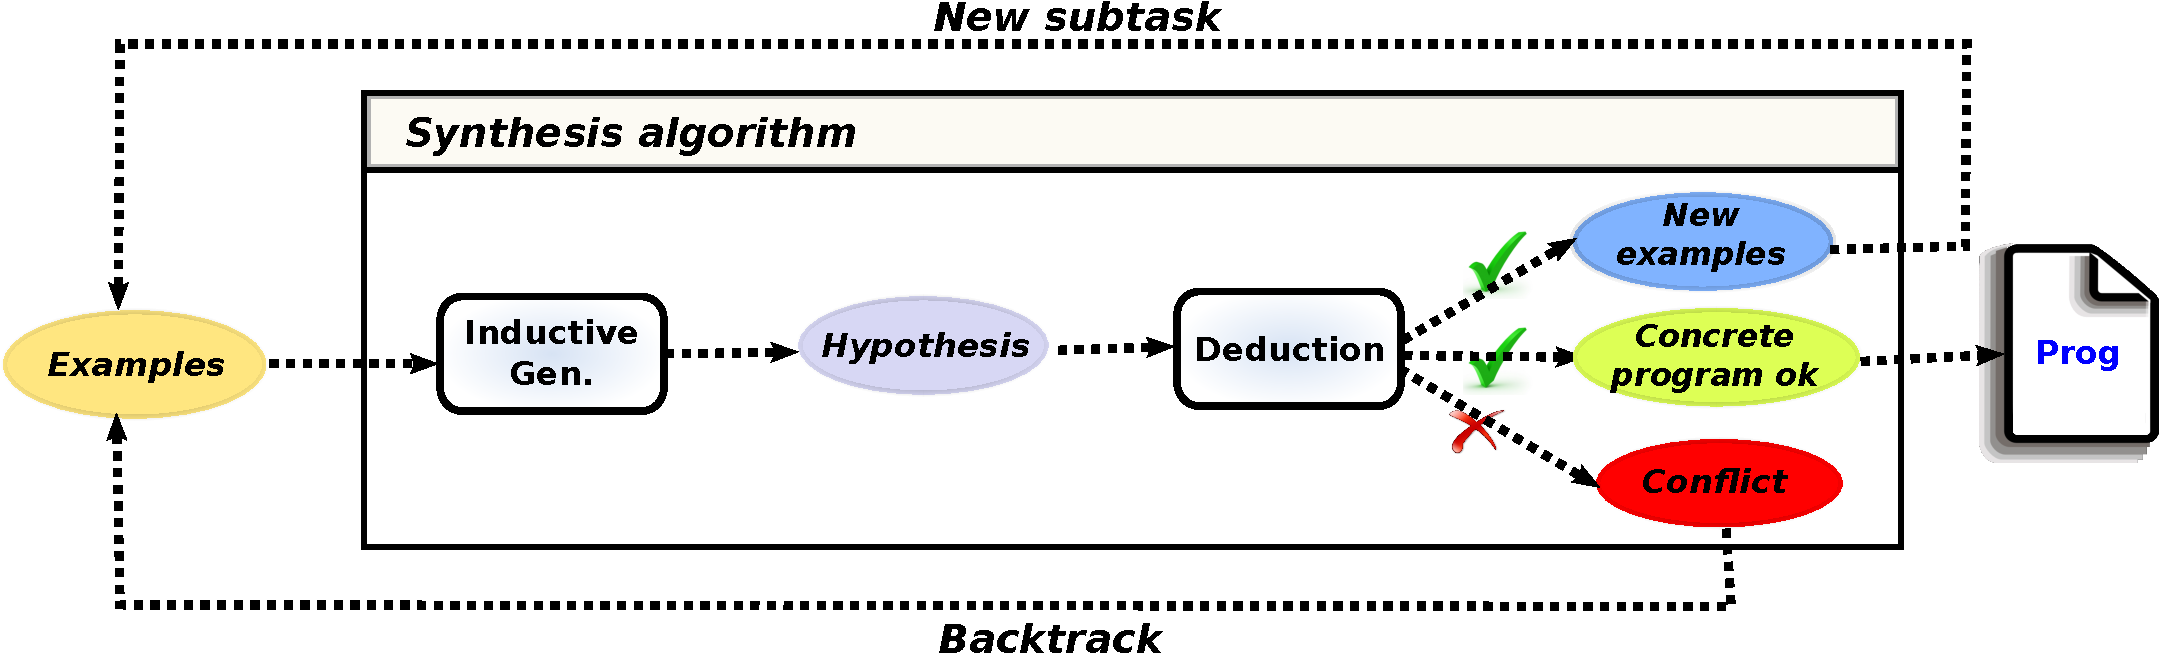
\includegraphics[scale=0.37]{overview-modified3.pdf}
\end{center}
\caption{High-level overview of our synthesis
  algorithm}\label{fig:overview}
\vspace{-0.1in}
\end{figure*}

\paragraph{Programming language} 

Our method synthesizes programs in a $\lambda$-calculus with algebraic
types and recursion. Let us consider {\em signatures} $\zug{\Op,
  \id{Const}, \cal{A}}$, where $\Op$ is a set of {\em primitive
  operators}, $\id{Const}$ is a set of constants, and $\cal{A}$ is a
set of equations that relate operators and constants.  The syntax of
programs $e$ over such a signature is given by:
\begin{eqnarray*} e & ::= & x \mid c \mid \lambda x. e' \mid e_1~e_2 \mid \rec~f.(\lambda x. e')
 \mid (e_1,e_2) \mid \oplus~e' \mid \\
 & & \{ l_1: e_1,\dots, l_k: e_k \} \mid e'.l \mid \zug{l_i(e_i)} \mid \\
  & & \matchc~e'~\withc~\zug{l_1(x_1) \Rightarrow
    e_1',\dots, l_k(x_k) \Rightarrow
    e_k'} 
\end{eqnarray*}

Here, $x$ and $f$ are variables, $\oplus \in \Op$, and $c \in \id{Const}$.
% is a {\em primitive
%  operator} and $c$ is a {\em constant}. Operators and constants are
%assumed to be related by an equational theory that rules, for
%instance, that $2 + 2 = 4$. 
The syntax has standard meaning; in particular:
\begin{enumerate}
\item $\rec~f.(\lambda x. e)$ is a recursive function $f$.

\item $e = \{ l_1: e_1,\dots, l_k: e_k \}$ is a record whose
field $l_i$ has value $e_i$. We have $e.l_i = e_i$.

\item $e = \zug{l_i(e_i)}$ is a variant labeled $l_i$. The construct
  ``$\matchc~e~\withc~\dots$'' performs ML-style pattern-matching. 
\end{enumerate}
We assume the standard definition of free variables. A
program is {\em closed} if it does not have any free variables.

As the operational semantics of the language is standard, we do not
discuss it in detail. We simply assume that we have a relation $\leadsto$
such that $e_1 \leadsto e_2$ whenever $e_1$ evaluates to $e_2$ in one
or more steps. 
%A program is {\em irreducible} if it does not evaluate
%to a program other than itself.
Our programs are typed using an ML-style polymorphic type system. Since this
system is standard,  we skip a detailed description.

Our implementation of the language comes prepackaged with certain
primitive operators, constants, and type definitions. Predefined types
include (polymorphic) lists and trees, encoded as variants.
Predefined operators include the standard arithmetic operators,
if-then-else, and higher-order combinators like {\tt map}, {\tt
  foldl}, {\tt foldr}, and {\tt foldt} (see Figure~\ref{fig:abstract-hypotheses}). In a particular synthesis
task, we may augment this set with {\em external} operators, constants
and types. For instance, in the synthesis of the \verb+selectnodes+
function in \secref{selectnodes}, {\tt pr} is an external operator.


\newcommand{\C}{\mathcal{C}}
\paragraph{Cost model}

Each program $e$ in the language has a {\em cost} $\C(e) \ge 0$.  This
cost is defined inductively. Specifically, we assume that each
primitive operator $\oplus$ and constant $c$ has a known, positive
cost. Costs for more complex expressions satisfy constraints like the
following (we skip some of the cases for brevity):
\begin{itemize}
\item $\C(\oplus~e) > \C(\oplus) + \C(e)$
\item $\C(\lambda x. e) > \C(e)$ 
\item $\C(e_1~e_2) > \C(e_1) + \C(e_2)$
\item $\C(x) = 0$. Intuitively, we assign costs to the {\em definition},
  rather than the {\em use}, of variables.
\end{itemize}



\paragraph{The synthesis problem}

Let an {\em input-output example} be a term $a_i \mapsto b_i$, where
$a_i$ and $b_i$ are closed programs. The input to our synthesis
problem is a set $\E_{in}$ of such examples. Our goal is to
compute a {\em minimal-cost} closed program $e$ 
%(often called the {\em target program}) 
that {\em satisfies} the examples --- i.e., for each $i$, we have $(e~a_i)
\leadsto b_i$. In what follows, we refer to $e$ as the \emph{target program}.

Note that this problem formulation biases our synthesis procedure towards
generating simpler programs. For example, since our implementation associates a higher cost 
with the {\tt match} %$\matchc~\dots~\withc~\dots$ 
construct than the \verb+fold+ %and \verb+foldr+
operators, our implementation favors fold-based implementations of list-transforming programs
over those that use pattern-matching.

%As an example, our implementation is
%designed to favor fold-based implementations of functions over lists
%over ones that use explicit pattern-matching. This is done by setting
%the cost for our ``$\matchc~\dots~\withc~\dots$'' construct to be
%adequately higher than the costs of the \verb+foldl+ and \verb+foldr+
%operators.

\paragraph{Hypotheses} The concept of {\em hypotheses} about the
structure of the target programs is key to our approach. Intuitively,
a hypothesis is a program that may have placeholders for missing
expressions. Formally, a {\em hypothesis} is a program that possibly
has free variables. Free variables in a hypothesis are also known as
{\em holes}, and a hypothesis with holes is said to be {\em open}. For
instance, $x$ and $\lambda x. f^* x$ are open hypotheses. In contrast, 
hypotheses that do not contain free variables are said to be \emph{closed}. 
For example, $\lambda x. \ {\tt map} \ (\lambda y. \ y+1) \ x$ is a closed hypothesis.

A hypothesis $h$ is typed under a {\em typing context} that assigns
types to its holes. Given a type $\tau$, we say that $h$ is {\em
  consistent} with $\tau$ if there exists a typing context under which
the type of $h$ equals $\tau$. This property can be decided using a 
standard type inference algorithm.


\section{Synthesis algorithm}\seclabel{algo}


\begin{comment}
\begin{figure*}[t]
\vspace{-0.15in}
\begin{center}
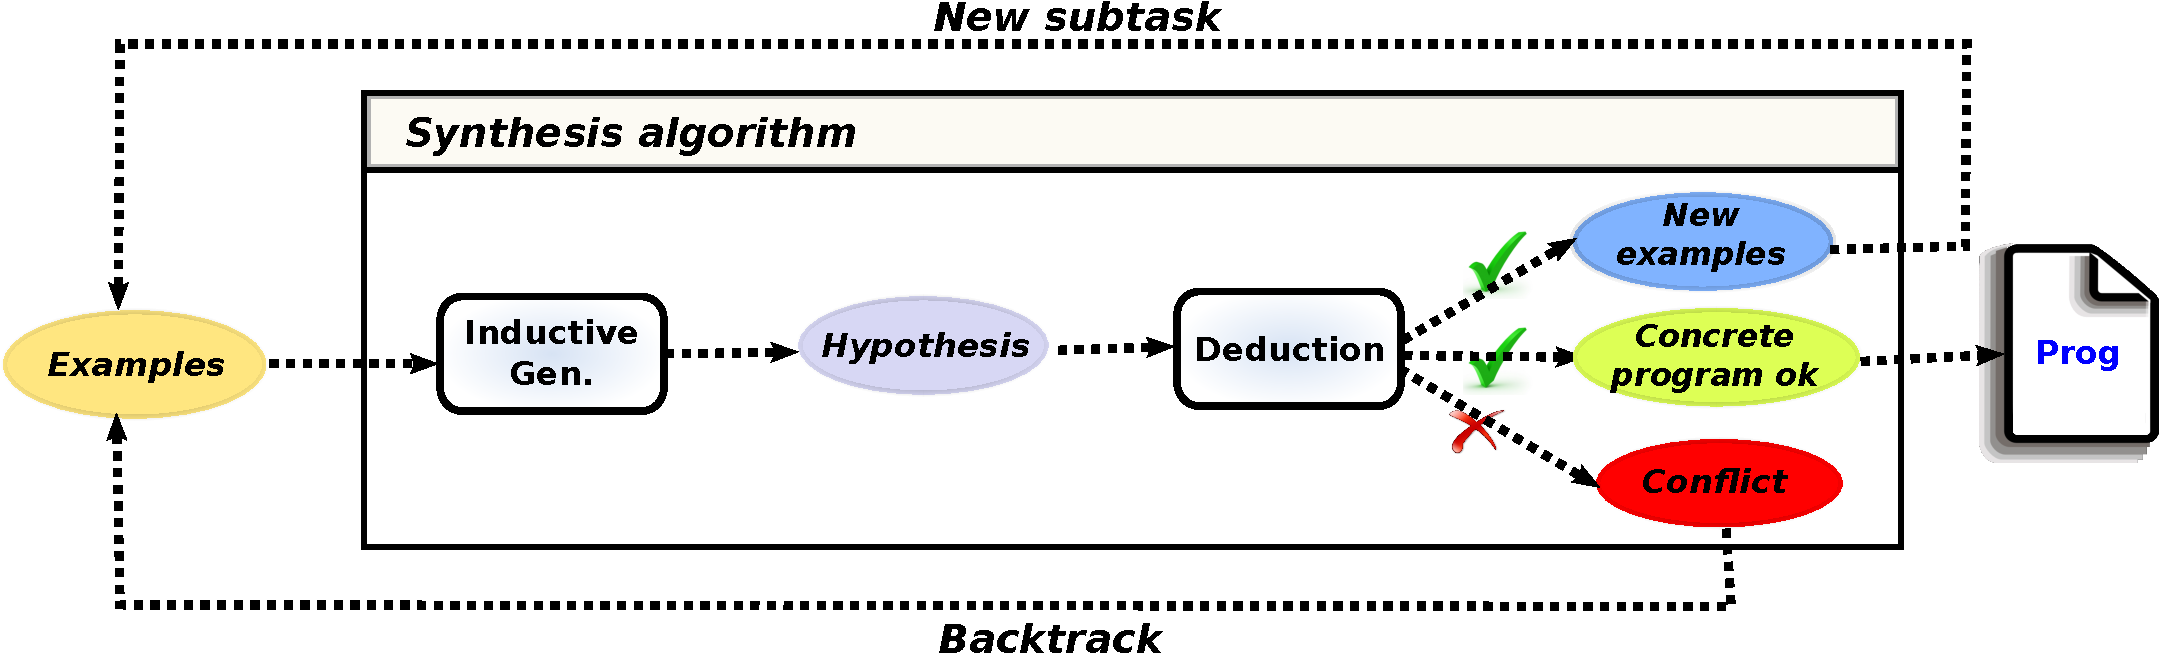
\includegraphics[scale=0.37]{overview-modified3.pdf}
\end{center}
\caption{High-level overview of our synthesis
  algorithm}\label{fig:overview}
\vspace{-0.1in}
\end{figure*}
\end{comment}

This section describes our procedure for solving the synthesis problem
from \secref{problem}.

\subsection{Algorithm architecture}\label{sec:overview}


Our synthesis procedure performs an \emph{enumerative search} that
interleaves \emph{inductive generalization} and \emph{deductive
  reasoning}. Specifically, the procedure maintains a priority queue
$Q$ of {\em synthesis subtasks} of the form $(e, f, \E)$, where $e$ is
a hypothesis, $f$ is a hole in the hypothesis, and $\E$ is a set of
examples. The interpretation of such a task is:
\begin{quote}
  Find a replacement $e^*$ for the hole $f$ such that $e^*$ satisfies
  the examples $\E$, and the program $e[e^*/f]$ obtained by
  substituting $f$ by $e^*$ satisfies the top-level input-output
  examples $\E_{in}$.
\end{quote}

The procedure iteratively processes  subtasks in the \emph{task pool} $Q$. \figref{overview} 
gives an overview of our strategy for solving each subtask $(e, f, \E)$.
First, our algorithm performs inductive generalization over  examples $\E$ to
produce a lazy stream of hypotheses $H$ about candidates $e^*$ that can  replace $f$.
As mentioned earlier, these hypotheses are
generated in a {\em type-aware} way, meaning that we %we infer the type
%$\tau$ of the target program from $\E$ and
rule out hypotheses that
are inconsistent with the inferred type $\tau$ of examples $\E$.



Next, for each hypothesis $h$ in $H$, our algorithm applies \emph{deductive
  reasoning} to check for potential {\em conflicts}. If the hypothesis
is closed, then a conflict arises if $e$ does not satisfy the
top-level (user-provided) input-output examples $\E_{in}$. 
In this case, the procedure
simply picks a new synthesis subtask from the task pool $Q$.
This corresponds to a form of \emph{backtracking} in the overall algorithm.

If the hypothesis is open, a conflict indicates that the provided
input-output examples violate a known axiom of a primitive operator
used in the hypothesis (i.e., there is {\em no way} in which the
hypothesis can be successfully completed). Upon conflict detection,
our procedure again backtracks and considers a different inductive
generalization.

If  hypothesis $h$ is open and no conflicts are found, the procedure generates new subtasks for
each hole $f$ in $h$ and uses deduction to learn new
input-output examples. In more detail, each new subtask is of the
form $(e', f^*, \E^*)$ where $e'$ is a new hypothesis, $f^*$ is a
new hole to be synthesized, and $\E^*$ is the set of inferred
input-output examples for $f^*$. This new subtask is now added to the task pool $Q$.

The procedure terminates once the search selects a subtask where the
hypothesis is closed and which does not conflict with the top-level
examples $\E_{in}$. 


 
%%%%%%%%%%%%%%%%%


 % \begin{figure}[!t]
% {\small 
%    \begin{tabbing}
%      mmm\=mmm\=mmm\=mmm\=mmm\=\kill
%      procedure {\sc Synthesize}($f, E, P, E'$):\\
    
%      \> input:  I/O examples $E$ for unknown function $f$, \\ 
%           \> \ \ \ \ \ \ \ \ \ \   program $P$ synthesized so far, and  \\
%      \> \ \ \ \ \ \ \ \ \ \ I/O examples $E'$ for the top-level synthesis problem \\
%      \> output: a program $P'$ if synthesis succeeds, $\bot$ otherwise \\
%      \> \\
%      \> (1) \> let $\tau$ := {\sc TypeInfer}$(E)$ in \\
%      \> (2) \> let $H$ := {\sc InductiveGen}($\tau$) in \\
%      \> (3) \> foreach $h \in H$: \\
%      \> (4) \> \ \ \ \ let $P'$ := $P[h/f]$ in  \\
%      \> (5) \> \ \ \ \ foreach $f^\star \in {\rm holes}(H)$: \\
%      \> (6) \> \ \ \ \ \ \ \ \  let $E^\star$ := {\sc Deduce}($h, f^*, E$) in \\
%      \> (7) \> \ \ \ \ \ \ \ \ if($E^\star = \bot$) break; \\
%      \> (8) \> \ \ \ \ \ \ \ \ let $P^\star$ := {\sc Synthesize}($E^\star, f^\star, E', P'$) in \\
%      \> (9) \> \ \ \ \ \ \ \ \ if($P^\star = \bot$) break; \\
%      \> (10) \> \ \ \ \ \ \ \ \ $P' := P[P^\star/f^\star]$ \\
%      \> (11) \> \ \ \ \ if({\sc Consistent}($P', E'$)) return $P'$ \\
%      \> (12) \> return $\bot$
%    \end{tabbing}
% } 
%    \caption{DO NOT TOUCH: Old synthesis algorithm}
%    \label{fig:algorithm}
%  \end{figure}
 
 
 % \todo{If we want to guarantee optimality, we need to change this
 % algorithm. Maybe pass a value $k$ to Synthesize and InductiveGen.
 % In that case, Synthesize and Inductive Gen also need to return an
 % integer that indicates the size of synthesized expression. }
 
 \figref{algorithm} gives pseudocode for the overall synthesis algorithm. Here, $Q$ is a \emph{priority queue} of
 tasks $(e, f, \E)$ sorted according to the cost of hypothesis $e$. In each iteration of the outer loop, we pick
 a \emph{minimum-cost} subtask $(e, f, \E)$ from task pool $Q$. Now, if $e$ is a closed hypothesis, 
 we use the
 routine {\sc Consistent} at line 5 to deductively check whether $e$ satisfies examples $\E_{in}$. If  this is the case,
$e$ must be a minimum-cost implementation consistent with $\E_{in}$; hence we return  $e$ as a solution to the synthesis problem. On the other
hand, if $e$ is not consistent with $\E_{in}$, we continue with a different candidate in the task pool $Q$.



 \begin{figure}[!t]
{\small 
%In tuples (h, f, Ex, Ex'), h is a hypothesis, f is a hole in it, Ex
%is examples for f, and Ex' is examples at top-level \\ 
\begin{algorithm}{Synthesize}{\E_{in}} 
Q \= \{ (f, f, \E) \}   \qquad \text{// $f$ is a fresh variable name }    \\
\begin{WHILE}{Q \ne \emptyset}
      \textrm{pick }(e, f, \E) \textrm{ from }Q \textrm{ such
        that }e\textrm{ has minimal cost}\\
      \begin{IF}{e~\textrm{is closed}}
           \begin{IF}{\CALL{Consistent}(e, \E_{in})} 
                  \RETURN e 
            \ELSE \textbf{continue}
           \end{IF} 
       \end{IF}\\
      \tau \= \CALL{TypeInfer}(\E) \\
      H \= \CALL{InductiveGen}(\tau) \\
      \begin{FOR}{h \in H}   
           e' \= e[h/f] \\
           \begin{IF}{e' \textrm{is closed}}    
              Q \= Q \cup \{ (e',\bot , \emptyset)  \} 
	      \ELSE 
	        \begin{FOR}{f^* \in \CALL{Holes}(e')}
                \E^* \= \CALL{Deduce}(e', f^*, \E) \\
                \textbf{if}~\E^* = \ \perp~\textbf{then break} \\
                %\begin{IF}{\E^* = \perp}\textbf{break} \end{IF} \\
                Q \= Q \cup \{ (e', f^*, \E^*) \} 
             \end{FOR}
           \end{IF}
       \end{FOR}
\end{WHILE} \\
\RETURN \perp
\end{algorithm}
} 
\vspace{-0.2in}
\caption{Synthesis procedure. %$\E_{in}$ is a set of
  %user-provided input-output examples
  }
   \label{fig:algorithm}
\vspace{-0.1in}
 \end{figure}

 Now, if $e$ is an open hypothesis, we still need to synthesize the free variable $f$ in $e$. 
 For this purpose, we use the {\sc TypeInfer} procedure at line 8 to infer 
 the type of $f$ from examples $\E$ and then call {\sc
   InductiveGen} to perform type-aware inductive generalization. % of examples $\E$.
  Suppose $H$ is a list of possible inductive generalizations for $f$. Now, we obtain a new hypothesis $e'$ by 
  replacing $f$ with a hypothesis $h \in H$. If $e'$ is closed, there are no new 
  unknowns to synthesize; hence, we add a single subtask $(e', \bot, \emptyset)$ to the task pool $Q$. 
  
  
  On the other hand, if $e'$ is  an open hypothesis, we generate new subtasks for synthesizing each hole in $e'$. Here, the procedure  {\sc Deduce} infers new examples for a specified hole $f^*$ in $e'$. 
  If a conflict is detected (i.e., $e'$ is not consistent with a known axiom), then {\sc Deduce} returns $\perp$, which
causes  backtracking from the current hypothesis. If no conflicts are detected, we add new subtasks of the form $(e', f^*, \E^*)$
to~$Q$.

 % conflicts with
 %axioms for operators (in this case, it returns $\perp$), and computes
 %new examples for a specified hole in the hypothesis.

 \begin{comment}
 Note that, in each iteration of the main loop, our synthesis algorithm picks a
 subtask $(e, f, \E)$ where the cost of $e$ is minimal among all
 available choices. We show in \secref{optimality} that this strategy
 guarantees optimality of synthesis.
\end{comment}

\subsection{Hypothesis Generation}\label{sec:ind-gen}

% As mentioned earlier, our algorithm generates two kinds of
% hypotheses: (i) concrete programs, and (ii) program skeletons with
% holes. From now on, we will refer to the first kind of hypothesis as
% a \emph{concrete hypothesis} and to the latter as an \emph{abstract
% hypothesis}. Our abstract hypotheses are drawn from a family of
% combinators that involve higher-order functions and that are
% commonly used to implement data structure transformations (e.g.,
% {\tt filter}, {\tt fold} etc.)
This section explains the hypothesis generation step of the synthesis algorithm in more detail.


The first step of inductive generalization is to decide if we
want to generate a closed or open hypothesis.  Since open hypotheses
are used to encapsulate common data structure transformation patterns,
we only introduce them when the input
examples correspond to recursive data structures. In particular, if
the inferred type of the transformation is $\tau_1 \rightarrow \tau_1$
and $\tau_1$ and $\tau_2$ are primitive types (e.g., ${\tt int}
\rightarrow {\tt int}$), then our procedure only generates closed
hypotheses.
% ~\footnote{Our current implementation also has a fixed depth limit
% beyond which it only generates concrete hypotheses.}


\begin{figure*}
{\small 
\begin{center}
\begin{tabular}{|c|l|}
\hline 
Hypothesis &  Definition of Combinator  \\ \hline
$\lambda x. \ \mathtt{map} \ f \ x$ & 
\begin{tabular}{l} 
  ${\tt map}$ \ :: $(a \rightarrow b) \rightarrow {\tt list}[a]  
  \rightarrow {\tt list}[b]$  \\
  ${\tt map}$ \ $f\ [\ ]  = [ \ ] $ \\
  ${\tt map}$ \ $f\ (x:y)  = (f \ x):({\tt map}\  y \ f) $ 
 \end{tabular}  
   \\ \hline
  $\lambda x. \ {\tt mapt} \ f \ x $ &
  \begin{tabular}{l} 
  ${\tt mapt}$ \ :: $ (a \rightarrow b) \rightarrow {\tt tree}[a] \rightarrow {\tt tree}[b]$  \\
  ${\tt mapt}$ \ $f\ {\tt tree}()  = {\tt tree}()$  \\
  ${\tt mapt}$ \ $f\ {\tt tree}(x, y) = {\tt tree}(f \ x,\ {\tt
    mapt} \ f \ y)$  \\
 \end{tabular}  \\ \hline
 $\lambda x. \ {\tt filter} \ f \ x$ & 
  \begin{tabular}{l} 
  ${\tt filter}$ \ :: $(a \rightarrow {\tt bool}) \rightarrow {\tt list}[a] \rightarrow {\tt list}[a]$  \\
  ${\tt filter}$ \ $f\ [\ ] = [ \ ] $ \\
  ${\tt filter}$ \ $(x:y)  \ f = \mathrm{if}~f \ x\ \mathrm{then} \
  x:({\tt filter}\ f \ y)  \  \mathrm{else} \  {\tt filter} \  f \ y$
 \end{tabular} 
 \\
\hline
$\lambda x. \ {\tt foldl} \ f \ e\ x$ & 
  \begin{tabular}{l} 
  ${\tt foldl}$\ :: $(b \rightarrow a \rightarrow b) \rightarrow b \rightarrow {\tt list}[a]  \rightarrow b$  \\
  ${\tt foldl}$ \ $f \ e\ [\ ]= e $ \\
  ${\tt foldl}$ \ $f\ e\ (x:y) =  {\tt foldl}  \ f \ (f \ e \ x)\ y$ \\
 \end{tabular} 
\\ \hline
$\lambda x. \ {\tt foldr} \ f \ e \ x$ & 
  \begin{tabular}{l} 
  ${\tt foldr}$\ :: $(b \rightarrow a \rightarrow b) \rightarrow b \rightarrow {\tt list}[a]  \rightarrow b$  \\
  ${\tt foldr}$ \ $f \ e\ [\ ]  = e $ \\
  ${\tt foldr}$ \ $f \ e\ (x:y) = f \ ({\tt foldr} \ f \ e\ y) \ x$ \\
 \end{tabular} 
\\  \hline 
 $\lambda x. \ {\tt foldt} \ f \ e\ x$ & 
  \begin{tabular}{l} 
  ${\tt foldt}$\ :: $({\tt list}[b] \rightarrow a \rightarrow b)
  \rightarrow b \rightarrow {\tt tree}[a] \rightarrow b$  \\
  ${\tt foldt}$ \ $f \ e\ {\tt tree}() = e$  \\
  ${\tt foldt}$ \ $f \ e\ {\tt tree}(x, y) = f \ ( {\tt map}\ (\lambda
  z. \  {\tt foldt} \ f \ e \ z)\ y) \ x$ \\
 \end{tabular}  \\
 \hline 
 
  $\lambda x. \ {\tt recl}\ f \ e\ x$ & 
  \begin{tabular}{l} 
    ${\tt recl}$\ :: $(a \rightarrow {\tt list}[a] \rightarrow b) \rightarrow b \rightarrow {\tt list}[a] \rightarrow  b$   \\
  ${\tt recl} \  f \ e\  \emptylist = \ e $  \\
  ${\tt recl}\ f \  e \ (x: y)  = \ f \  x \ y $ \\
 \end{tabular}  \\ \hline
\end{tabular}
\end{center}
}
\vspace{-0.1in}
\caption{Family of combinators from which we draw our open
  hypotheses. 
  %In the last definition,  function $f$  may refer to {\tt
   % recl}.
   } 
\label{fig:abstract-hypotheses}
\vspace{-0.1in}
\end{figure*}


The open hypotheses are drawn from the family of combinators shown in
\figref{abstract-hypotheses}. The first column of
\figref{abstract-hypotheses} shows the hypothesis which serves as our
inductive generalization, and the second column shows the definition
of the combinator used in the hypothesis. Observe that the free
variables in the first column correspond to new 
synthesis subproblems.
%For instance, if our inductive generalization is an open
%hypothesis of the form $\lambda x. \ \mathtt{map} \ f \ x$, our
%procedure must recursively synthesize an implementation for free
%variable $f$ used in this hypothesis.

Open hypothesis generation is guided by the inferred type of the
input-output examples. For instance, suppose we have the 
examples $\{ 
[\ ] \mapsto 0, [1] \mapsto 1, [1,2] \mapsto 3  \}$.
%$$
%[\ ] \mapsto 0 \qquad~~~ [1] \mapsto 1 \qquad~~~ [1,2] \mapsto 3
%$$
% \[
% \begin{array}{ccc}
%  [ \ ] & \rightarrow  & 0 & & 
% {\rm [ 1 ]} & \rightarrow & 1 \\
% {\rm [ 1, 2 ]} & \rightarrow & 3
% %[ 1 ] \rightarrow 1 
% %[1, 2] \rightarrow 3
% \end{array}
% \]
Here, since the inferred type of the transformation is $\mathtt{list}[
\mathtt{int}] \rightarrow \mathtt{int}$, our hypothesis generator
immediately rules out the first three combinators from
\figref{abstract-hypotheses} from being possible
generalizations. The use of types to guide generalization is
an important feature of our procedure and greatly helps to keep the
search space manageable (see ~\secref{eval}).

%In particular, using types to guide the
%generation of closed hypothesis is a significant performance
%improvement, as shown in Figure~\ref{fig:timing}.

If the inferred type of the input-output examples is not compatible
with any of the open hypotheses from \figref{abstract-hypotheses},
%or if the recursion depth exceeds some pre-determined threshold,
our synthesis procedure instead generates closed hypotheses. This is done by lazily
enumerating a stream of candidate expressions %(closed hypotheses) 
that
are compatible with the inferred type of the input-output
examples. The enumeration procedure generates the candidate expressions in increasing
order of cost.

Our hypothesis generator also uses a rewrite system to avoid
enumerating syntactically distinct but semantically equivalent
hypotheses. Given a candidate hypothesis $e$, this rewrite system
produces either the original hypothesis $e$ or an equivalent, but
lower-cost hypothesis $e'$. As our goal is to find a minimal-cost
program, we can safely prune $e$ from the search space in the latter
case.
For example, suppose our signature has addition as a primitive operator, 1
and 0 as constants, and the axiom $\forall x. x + 0 = 0 + x = 1$. In
this case, our rewrite system will make sure that $(1 + 0)$ is not
generated as a closed hypothesis. 

% Since the enumeration procedure is complete, whenever the rewrite
% system produces a lower-cost expression $e'$, this means that
% expression $e$ has already been explored; hence, we can safely prune
% $e$ from the search space.

% This pruning strategy greatly reduces the search space in
% practice. In particular, since our closed hypothesis generator
% recursively enumerates all expressions of type $t$ in a top-down
% fashion, pruning a single expression of type ${\rm list[int]}$
% allows our algorithm to prune a large number of expressions of type
% {\rm int}.


\begin{comment}
\todo{SC: I don't like this example too much. I'll fold this into
  the text on optimality.}

\begin{example}
  %The enumeration procedure starts with a set $I$ of expressions of
  %size 1 and a set of operators. To enumerate expressions of type
  %$\tau$, we first enumerate all expressions of type $\tau$ in
  %$I$. Next, we recursively apply operators to the expressions in $I$
  %to generate larger expressions. 
  Consider the enumeration of all expressions of type {\tt int} where
  the only expressions of size $1$ are $0, 1$, and $x$. Further,
  suppose that the only operator allowed on {\rm Int}'s is $+$. In
  this case, our procedure (with pruning) will generate the following
  stream: $0, 1, x, 1 + 1, 1 + x, x+x\dots$.
  
  
  %following stream will be generated: $0, 1, x, 0 + 0, 0 + 1, 0 + x, 1
  %+ 0, 1 + 1, 1 + x, \dots$. After pruning, the stream will be: $0, 1,
  %x, 1 + 1, 1 + x, \dots$.

  % Consider the enumeration of all expressions of type {\rm int}. As
  % part of the enumeration, we select all operators whose return
  % types unify with {\rm int} (i.e. Plus, Minus, Car, If). If the
  % operator has a polymorphic return type, we unify it with {\rm Int}
  % to get a substitution, and apply that substitution to the operator
  % type. For instance, {\rm If} is of type $bool \rightarrow a
  % \rightarrow a \rightarrow a$. Unifying $a$ with {\rm Int} returns
  % the substitution $[a: {\rm Int}]$ and applying that substitution
  % to the type of {\rm If} yields $bool \rightarrow {\rm Int}
  % \rightarrow {\rm Int} \rightarrow {\rm Int}$. Now that we have
  % operator types that are specialized for the correct return type,
  % we can search for arguments to these operators.

  % To search for operator arguments, we recursively call the
  % expression enumeration procedure to obtain streams for each
  % argument type. These streams are combined into a single stream of
  % argument lists using the composition operator defined by
  % Spivey. This process is performed for each selected operator and
  % the streams are merged to produce a stream of expressions of type
  % {\rm Int}.

  % Now it should be clearer why pruning expression streams is
  % valuable, even if it can only discard expressions that are already
  % generated. Generating an expression stream for type {\rm Int}
  % requires an expression stream for types {\rm Bool} and {\rm Int},
  % among others. Any pruning that can be performed significantly
  % reduces the total number of expressions that will be tested.
\end{example}
\end{comment}

\subsection{Inference of new examples using deduction}\seclabel{deduction}

%When the hypothesis generator produces an abstract hypothesis, our algorithm must recursively synthesize one or more unknown %functions that are used in the program skeleton. Furthermore, since the {\sc Synthesize} procedure from %Figure~\ref{fig:algorithm} requires input-output examples, we must construct new  examples characterizing the unknown %functions used in the skeleton. This task is accomplished using the {\sc Deduce} procedure used at line 6 of the {\sc %Synthesize} algorithm in Figure~\ref{fig:algorithm}. In this section, we  describe the core ideas underlying the {\sc Deduce} %procedure for generating new input-output examples characterizing the recursive subproblems.

We now explain the {\sc Deduce} procedure used in the synthesis algorithm
from Figure~\ref{fig:algorithm}.
Recall that {\sc Deduce} is used for 
inferring new input-output examples and detecting conflicts.
The deduction procedure used in our synthesis algorithm is \emph{sound} but \emph{incomplete}. In this context, we
define {soundness} and {completeness} as follows:

\begin{definition}{\bf (Soundness of deduction)} Let $\E$ be a set of
  input-output examples, and let $h$ be a hypothesis that is an
  inductive generalization of $\E$.  The {\sc Deduce} procedure is
  sound, if for every unknown $f$ in $h$, whenever {\sc Deduce}($h, f,
  \E$) = $\E'$ and the synthesis problem defined by $\E'$ and $f$ does
  not have a solution, then the synthesis problem defined by $\E$ and
  $h$ also does not have a solution.
\end{definition}

In other words, the deduction procedure is sound if the non-existence
of a solution to any  synthesis subtask implies the
non-existence of a solution to the original problem. Hence, soundness
implies that deduction will never cause our synthesis
procedure to reject a valid open hypothesis. However, since our
deduction procedure is not complete, the existence of a solution to
all  synthesis subtasks does not imply the existence of a
solution to the original problem. More technically, we define
{completeness} as follows:

\begin{definition}{\bf (Completeness of deduction)} Let $\E$ be a set of
  examples, and let $h$ be a hypothesis that is an inductive
  generalization of $\E$.  The completeness of {\sc Deduce} means that,
  if the synthesis problem defined by $\E, h$ does not have a solution,
  then there exists some unknown $f$ in $h$ such that (i) {\sc Deduce}($h,
  f, \E$) = $\E'$ and (ii) the synthesis problem defined by $\E', f$ does not
  have a solution.
\end{definition}

A consequence of incompleteness is that our synthesis procedure must
check that a closed hypothesis is consistent with the
user-provided example set $\E_{in}$. This is done in line 5 of the
{\sc Synthesize} procedure in Figure~\ref{fig:algorithm}.


\begin{figure*}
{\small 
\[
\begin{array}{c}
\irule{
\begin{array}{c}
\E = \bigcup_{1 \leq i \leq n} \{ [a_{i1}, \ldots, a_{ig(i)}] \mapsto  [b_{i1}, \ldots, b_{ih(i)}] \} \\
\exists i. (1 \leq i \leq n \land g(i) \neq h(i))
 \end{array}
}{\E, \lambda x. \ {\tt map} \ f\ x \vdash f: \bot } \qquad \qquad 

\irule{
\begin{array}{c}
\E = \bigcup_{1 \leq i \leq n} \{ [a_{i1}, \ldots, a_{ig(i)}] \mapsto  [b_{i1}, \ldots, b_{ih(i)}] \} \\
\exists i, j, k, m. \left ( 
\begin{array}{c} 
1 \leq i \leq n \land 1 \leq j \leq n \land 1 \leq k \leq g(i) \land \\ 1 \leq m \leq h(j)
\land a_{ik}  =  a_{jm} \land b_{ik} \neq b_{jm})
\end{array}
\right )
 \end{array}
}{\E, \lambda x. \ {\tt map} \ f \ x\vdash f: \bot } \\ \ \\ 

\irule{
\begin{array}{c}
\E = \bigcup_{1 \leq i \leq n} \{ [a_{i1}, \ldots, a_{ig(i)}] \mapsto  [b_{i1}, \ldots, b_{ig(i)}] \} \\
\E' = \bigcup_{1 \leq i \leq n} \{ a_{i1} \mapsto b_{i1}, \ldots  a_{ig(i)} \mapsto b_{ig(i)}\} \\
 ( (a, b) \in \E' \land (a', b') \in \E' \land a = a') \Rightarrow b = b'
 \end{array}
}{\E, \lambda x. \ {\tt map} \ f\ x \vdash f: \E'} \qquad \qquad  

\irule{
\begin{array}{c}
\E = \bigcup_{1 \leq i \leq n} \{ s_i \mapsto t_i \} \\
\exists i. (1 \leq i \leq n \land s_i \not\simeq t_i) \\
 \end{array}
}{\E, \lambda x. \ {\tt mapt} \ f\ x \vdash f: \bot } \\ \ \\  

\irule{
\begin{array}{c}
\E = \bigcup_{1 \leq i \leq n} \{ s_i \mapsto t_i \} \\
\exists i, j, k, m. \left ( 
\begin{array}{c} 
1 \leq i \leq n \land 1 \leq j \leq n \land 1 \leq k \leq {\rm size}(s_i) \land \\ 1 \leq m \leq {\rm size}(t_i)
\land s_{ik} = s_{jm} \land t_{ik} \neq t_{jm})
\end{array}
\right )
 \end{array}
}{\E, \lambda x. \ {\tt mapt} \ f \ x \vdash f: \bot } \qquad 

\irule{
\begin{array}{c}
\E = \bigcup_{1 \leq i \leq n} \{ s_i \mapsto t_i \} \qquad  k = {\rm size}(s_i) = {\rm size}(t_i) \\
\E' = \bigcup_{1 \leq i \leq n} \{ s_{i1} \mapsto t_{i1}, \ldots  s_{ik} \mapsto t_{ik}\} \\
 ( (a, b) \in \E' \land (a', b') \in \E' \land a = a') \Rightarrow b = b'
 \end{array}
}{\E, \lambda x. \ {\tt mapt} \ f \ x \vdash f: \E'} \\  \ \\

\irule{
\begin{array}{c}
\E = \bigcup_{1 \leq i \leq n} \{ [a_{i1}, \ldots, a_{ig(i)}] \mapsto  [b_{i1}, \ldots, b_{ih(i)}]  \} \\
\exists i. (1 \leq i \leq n \ \land \ h(i) > g(i)) 
\end{array}
}
{\E, \lambda x. \ {\tt filter} \ f \ x \vdash f: \bot}
\qquad \qquad 
\irule{
\begin{array}{c}
\E = \bigcup_{1 \leq i \leq n} \{ [a_{i1}, \ldots, a_{ig(i)}] \mapsto  [b_{i1}, \ldots, b_{ih(i)}]  \} \\
\exists i. \exists j. 1 \leq i \leq n \land 1 \leq j \leq g(i) \land \forall k. (k \geq j \Rightarrow b_{ij} \neq a_{ik})
\end{array}
}
{\E, \lambda x. \ {\tt filter} \ f \ x \vdash f: \bot}
\\ \ \\ 
\irule{
\begin{array}{c}
\E = \bigcup_{1 \leq i \leq n} \{ [a_{i1}, \ldots, a_{ig(i)}] \mapsto  [b_{i1}, \ldots, b_{ih(i)}]  \} \qquad \qquad 
\forall i. 1 \leq i \leq n \mapsto h(i) \leq g(i) \\
\forall (A \mapsto B) \in \E. \forall b_i \in B. \exists a_j \in A. (j \geq i \land b_i = a_j) \\
\E_T = \{ x \mapsto {\rm true} \ | \ x \in A \land x \in B \land A \mapsto B \in \E\} \qquad \qquad 
\E_F = \{ x \mapsto {\rm false} \ | \ x \in A \land x \not \in B \land A \mapsto B \in \E\} 
\end{array}
}
{\E, \lambda x. \ {\tt filter} \ f \ x \vdash f: \E_T \cup \E_F}

\end{array}
\]
}
\vspace{-0.1in}
\caption{Deductive reasoning for {\tt map},  {\tt mapt}, and {\tt filter}}\label{fig:deduce-map-filter}
\vspace{-0.1in}
\end{figure*}

We  now describe the deduction engine underlying our procedure as
inference rules of the form $
\E, h \vdash f: \E' $.
The meaning of this judgment is that, if $\E$ is a set of input-output
examples with inductive generalization $h$, then $\E'$ is a new set of
input-output examples for unknown $f$ used in expression $h$. Here,
$\E'$ may also be $\bot$, indicating that a conflict is detected and
that the subproblem defined by $f$ does not have a
solution. Note that the soundness of deduction implies that, if $\E, h
\vdash f: \bot$, then $h$ cannot be a correct inductive generalization
for examples $\E$.

%Since the inferred examples depend on the ``shape'' of  the abstract hypothesis, we have a custom deduction procedure for each different inductive generalization shown in Figure~\ref{fig:abstract-hypotheses}. For instance, 
%

Figure~\ref{fig:deduce-map-filter} shows the deductive reasoning
performed for hypotheses involving the {\tt map}, {\tt mapt} and {\tt
  filter} combinators. The first three rules in
Figure~\ref{fig:deduce-map-filter} concern hypotheses involving {\tt
  map}.  Specifically, the first rule deduces a conflict if $\E$
contains an input-output example of the form $A \mapsto B$ such
that $A$ and $B$ are lists but their lengths are not equal.
Similarly, the second rule deduces $\bot$ if $\E$ contains a pair of
input-output examples $A \mapsto B$ and $A' \mapsto B'$ such
that $A_i = A'_j$ but $B_i \neq B'_j$. Since function $f$ provided as
an argument to the {\tt map} combinator must produce the same output
for a given input, the existence of such an input-output example
indicates the hypothesis must be incorrect. Finally, the third rule in
Figure~\ref{fig:deduce-map-filter} shows how to deduce new examples
for $f$ when no conflicts are detected. Specifically, for an
input-output example of the form $A \mapsto B$ where $A$ and $B$
are lists, we can deduce examples $A_i \mapsto B_i$ for function
$f$.




\begin{example}
  Consider the input-output examples $[1, 2] \mapsto [2, 3]$ and $[2,
  4] \mapsto [3, 5]$ and the hypothesis $\lambda x. \ {\tt map} \ f \
  x$. Using the third rule from Figure~\ref{fig:deduce-map-filter}, we
  deduce the following new examples for $f$: $\{ 1 \mapsto 2, 2
  \mapsto 3, 4 \mapsto 5 \}$.
\end{example}

\begin{example}
  Consider the input-output examples $[1] \mapsto [1]$ and $[2,1,4]
  \mapsto [2, 3, 7]$ and the hypothesis $\lambda x. \ {\tt map} \ f \
  x$.  We can derive a conflict using the second rule of
  Figure~\ref{fig:deduce-map-filter} because $f$ maps  input $1$ to
  two different values $1$ and $3$.
  % This reasoning is sound since no instantiation of the hypothesis
  % can result in an expression that is consistent with the provided
  % examples.
\end{example}

Since the rules for {\tt mapt} are  similar to those for {\tt map},
 we do not explain them in detail. We use the notation $s_i \not \simeq t_i$ to indicate that trees $s_i$
and $t_i$ have incompatible ``shapes''.

%The second rule is almost identical to the second rule for {\tt map}; for list examples, elements are numbered by index %whereas for trees, elements are numbered in breadth-first order. Similarly, the third rule for {\tt mapt} shows how to deduce $new examples in the same manner as they are deduced for {\tt map}.

The last three rules of Figure~\ref{fig:deduce-map-filter} describe
the deduction process for the {\tt filter} combinator. Since $\lambda
x. {\tt filter} \ f \ x$ removes those elements of $x$ for which
$f(x)$ evaluates to false, the length of the output list cannot be
greater than that of the input list. Hence, the first rule for {\tt
  filter} derives a conflict if there exists an example $A \mapsto B$
such that the length of list $B$ is greater than the length of list
$A$.  Similarly, the second rule for {\tt filter} deduces $\bot$ if
there is some element in list $B$ that does not have a corresponding
element in list $A$.  If no conflicts are detected, the last rule of
Figure~\ref{fig:deduce-map-filter} infers input-output examples for
$f$ such that an element $x$ is mapped to true if and only if it is
retained in output list~$B$.

\begin{example}
  Consider the input-output example $[1, 2] \mapsto [1, 2, 1, 2]$ and
  the hypothesis $\lambda x. \ {\tt filter} \ f \ x$. Our procedure
  deduces a conflict using the first rule for {\tt filter}.
\end{example}

\begin{example}
  Consider the input-output example $[1, 2, 3] \mapsto [1, 3, 2]$ and
  the hypothesis $\lambda x. \ {\tt filter} \ f \ x$. This time, our
  procedure deduces $\bot$ using the second rule for {\tt filter}.
\end{example}

\begin{example}
  Consider the examples $[1, 2, 3] \mapsto [2]$ and $[2,
  8] \mapsto [2, 8]$ and the hypothesis $\lambda x. \ {\tt filter} \ f
  \ x$. Using the last rule of Figure~\ref{fig:deduce-map-filter}, we
  derive the following examples for $f$: $\{ 1\mapsto \false, 2
  \mapsto \true, 3 \mapsto \false, 8 \mapsto \true \}$.
\end{example}

% \todo{Question for Jack: Should we not have another inference rule
% that deduces a conflict if $f(i)$ is mapped to
% both %true and false? If so, can you add this as an inference rule along with an explanation?}

We now describe the deductive reasoning performed for the {\tt
  foldl} and {\tt foldr} combinators (we collectively refer to these
operators as {\tt fold}).  Consider a hypothesis of the form
$\lambda x. \ {\tt fold} \  f \ e \ x$ and suppose we want to learn new
input-output examples characterizing $f$. We have found that deducing
new examples for $f$ in a sound and scalable way is only possible if the
expression $e$ is a constant, as oppposed to a function of
$x$. Therefore, our procedure generates two separate hypotheses
involving {\tt fold}:

\begin{enumerate}
\item $\lambda x. \ {\tt fold}  \ f \ c \ x$  where $c$ is a constant
\item $\lambda x. \ {\tt fold}  \ f \ e\ x$  where $e$ is an arbitrary expression.
\end{enumerate}

Our deduction engine can make inferences and generate useful examples
only for case (1).  The second case relies on enumerative search,
which is possible even without examples.  As new examples can prune
the search space significantly, synthesis is more likely to be
efficient in case (1), and we always try the first hypothesis before
the second one. In what follows, we discuss the inference rules for
{\tt fold} under the assumption that it has a constant base case.

Figure~\ref{fig:deduce-fold} describes the deduction process for
combinators involving {\tt foldl}, {\tt foldr} and {\tt rec} using set
inclusion constraints. Specifically, the set $\E'$ in these rules
denotes the smallest set satisfying the generated
constraints. Consider the first two rules of
Figure~\ref{fig:deduce-fold}. By the first rule, if there are two
input-output examples of the form $[\ ] \mapsto b$ and $[~] \mapsto
b'$ such that $b \neq b'$, this means that we cannot synthesize the
program using a fold operator with a constant base case; hence we
derive $\bot$. Otherwise, if there is an example $[~] \mapsto b$, we
infer the initial seed value for {\tt fold} to be $b$.

\begin{comment}
  While the deductive reasoning performed for the {\tt map} and {\tt
    filter} combinators is both sound and complete, the inference
  rules shown in Figure~\ref{fig:deduce-fold} for the {\tt fold} and
  general recursion ({\tt rec}) combinators are sound but incomplete.
  Figure~\ref{fig:deduce-fold} describes the deduction process for
  these combinators using set inclusion constraints. Specifically, the
  set $E'$ in these rules denotes the smallest set satisfying the
  generated constraints.

However, the inference rules for folds are only sound when the base
case for the fold is constant. If the base case is known to be
non-constant, examples can be inferred for $e$, but not for $f$. It is
not correct to assume that, because all provided examples have a
constant base case, the base case is constant in general. While it is
safe to assume a fixed base and deduce examples, in general we are
searching for a base case. 
\end{comment}


Let us now consider the  third rule (i.e., {\tt foldr}), and suppose  we have an example
$E_1: \ [a_1, \ldots, a_n] \mapsto b$ and another example $E_2: \ \ {\rm [}a_2, \ldots, a_n{\rm ]} \mapsto b' $.
%the following pair of input-output examples:
%\[
%\begin{array}{ll}
%E_1: \ \ [a_1, \ldots, a_n] \mapsto b \ \ \ & \ \ \  
%E_2: \ \ {\rm [}a_2, \ldots, a_n{\rm ]} \mapsto b' 
%\end{array}
%\]
Now, observe the following equivalences:
\[
\begin{array}{ll}
 {\tt foldr} \  f \ y\ [a_1, \ldots, a_n]  & \\
 \ \ \ \equiv   f \  ({\tt foldr} \ f \ y\ \ [a_2, \ldots, a_n]) \ a_1 & {\rm (def. \ of \  {\tt foldr})} \\
 \ \ \ \equiv f \   b' \ a_1  & {\rm (from}\  E_2) \\
 \ \ \ \equiv b & {\rm (from} \ E_1)
\end{array}
\]
Since we have  $f \ b' \ a_1 = b$, it is sound to deduce the input-output example $( b', a_1) \mapsto b$ for the unknown function $f$.

As shown in the fourth rule, we  can apply similar reasoning to {\tt foldl}. Suppose we have the following  examples:
\[
\begin{array}{ll}
E_1': \ \ [a_1, \ldots, a_n] \mapsto b  \ \ \  &  \ \ \ 
E_2': {\rm [}a_1, \ldots, a_{n-1}{\rm ]} \mapsto b' 
\end{array}
\]
We can again expand the recursive definition of {\tt foldl} to obtain the following equivalences:
\[
\begin{array}{ll}
 {\tt foldl}\ f \ y\ \ [a_1, \ldots, a_n]  & \\
 \ \ \ \equiv    f \ a_n\ ({\tt foldl} \ f \ y\ \  [a_1, \ldots, a_{n-1}])   & {\rm (property \ of \  {\tt foldl})} \\
 \ \ \ \equiv f \   a_n \ b'  & {\rm (from}\  E_2') \\
 \ \ \ \equiv b & {\rm (from} \ E_1')
\end{array}
\]
Hence, we can   infer the input-output example $(a_n, b') \mapsto b$ for function $f$. However, as illustrated by the following example, these inference rules are not complete.

\begin{figure}
{\small 
\[
\begin{array}{c}
  \irule{([] \mapsto b)  \  \in \E,  \ \ ([] \mapsto b')  \  \in \E,  \ \ b \neq b' }
  {\E, \lambda x. \ {\tt fold}\ f \ c\ x \vdash c: \bot} \\ \ \\ 
  \irule{ \ ([\ ] \mapsto b) \in \E}
  {\E, \lambda x. \ {\tt fold}\ f \ c\ x \vdash c: \{ b \}} \\ \ \\
  %\land E,
   % \lambda x. \ {\tt foldr} \ x \ f \ e \vdash e: E'} \\ \ \\
  \irule{
    \begin{array}{c}
     % (([\ ] \mapsto b) \in E \land ([\ ] \mapsto b') \in E) \Rightarrow b = b' \\
      ([a_1, \ldots, a_n] \mapsto b) \in \E \\
      ([a_2, \ldots, a_n] \mapsto b') \in \E \\
    \end{array}
  }{\E, \lambda x. \ {\tt foldr}\ f \ c\ x \vdash f: ((b', a_1) \mapsto b) \in \E'} \\ \ \\
  \irule{
    \begin{array}{c}
      %(([\ ] \mapsto b) \in E \land ([\ ] \mapsto b') \in E) \Rightarrow b = b' \\
      ([a_1, \ldots, a_n] \mapsto b) \in \E  \\
      ([a_1, \ldots, a_{n-1}] \mapsto b') \in \E \\
    \end{array}
  }{\E, \lambda x. \ {\tt foldl} \ f \ c\ x \vdash f: ((a_n, b') \mapsto b) \in \E'} \\ \ \\
  \irule{({\rm tree}() \mapsto b)  \  \in \E,  \ \ ({\rm tree}() \mapsto b')  \  \in \E,  \ \ b \neq b' }
  {\E, \lambda x. \ {\tt foldt}  \ f \ c\ x \vdash c: \bot} \\ \ \\ 
  \irule{ ({\rm tree}() \mapsto b) \in \E} 
  {\E, \lambda x. \ {\tt foldt}  \ f \ c \ x\vdash c: \{b\}} \\ \ \\

  \irule{
    \begin{array}{c}
     % (({\rm tree}() \mapsto b) \in E \land ({\rm tree}() \mapsto b') \in E) \Rightarrow b = b' \\
      {\rm tree}(a, [b_1, \ldots, b_n]) \mapsto c \in \E \\
      \forall i. (1 \leq i \leq n \Rightarrow (b_i \mapsto c'_i \in \E)) \\
    \end{array}
  }{\E, \lambda x. \ {\tt foldt} \ f \ c \ x\vdash f: ([c'_1, \ldots, c'_n], a) \mapsto c) \in \E'} \\ \ \\

  \irule{
    ( x:xs \mapsto b)  \in  \E
  }
  {\E, \lambda x. {\tt recl} \ f \ e \ x\vdash f: ((x, xs) \mapsto b) \in \E' }
\end{array}
\]
}
\vspace{-0.1in}
\caption{Deduction for {\tt fold} and general
  recursion.}\label{fig:deduce-fold}
  \vspace{-0.1in}
\end{figure}


\begin{example}
Consider the hypothesis $\lambda x. \ {\tt foldl} \ f \ y \ x$, and the following input-output examples provided by the user:
\[
\begin{array}{lll}
\emptylist \mapsto  0 & 
\mylist{1}  \mapsto  1 &
\mylist{1, 2}  \mapsto  3 \\
\mylist{2, 3} \mapsto 5 & 
\mylist{1, 2, 3} \mapsto 6 & 
\mylist{2,3,5} \mapsto 10
\end{array}
\]
Using the inference rules from Figure~\ref{fig:deduce-fold}, we infer the following input-output examples for $f$:
\[
(1, 0)  \mapsto 1, \ \ \ (2, 1) \mapsto 3, \ \ \  (3, 3) \mapsto 6, \ \ \ (5, 5) \mapsto 10
\]
Observe that  there is information provided by   $\mylist{2, 3} \mapsto 5 $ that is not captured by the inferred examples for~$f$.
\end{example}

The next three rules for {\tt foldt} are very similar to {\tt foldl} and {\tt foldr}; hence, we do not discuss them in detail.
The last rule in Figure~\ref{fig:deduce-fold} infers input-output examples for  function $f$ used in the general recursion combinator. Recall from Figure~\ref{fig:abstract-hypotheses} that, given an input list of the form $x:xs$, the general recursion combinator applies function $f$ to pair $(x, xs)$. Hence, for any input example of the form $[a_1, \ldots, a_n] \mapsto b$, we can deduce the example $(a_1, [a_2, \ldots, a_n]) \mapsto b$ for unknown function $f$.


\begin{comment}

\subsection{Extensions}
%\subsubsection{Example scopes}
\todo{I don't entirely understand this discussion. I think we need to
elaborate on this some more. --Isil}
In the implementation, IO examples are not the entire story. Given an
unknown function $f^*$, each example for $f^*$ is attached to a scope,
which contains value bindings that are accessible to the unknown
function. Consider the hypothesis $\lambda\ x.\ ${\tt map}$\ f^*\ x$
and the example $[1, 2] \mapsto [3, 4]$. When we deduce examples
for $f^*$, each example will be associated with the scope $\{x:[1,
2]\}$. When generalizing $f^*$, values in scope are considered in
addition to function arguments as possible inputs to a combinator. The
scope is considered to be part of the ``input'' side of the example,
so when comparing the left hand sides of two examples, the scopes are
compared as well as the inputs.

This has implications for the deduction rules. In particular, given
examples $a_1 \mapsto b_1$ and $a_2 \mapsto b_2$ and scopes
$s_1$ and $s_2$, we derive a conflict if and only if $a_1 = a_2 \land
s_1 = s_2 \land b_1 \neq b_2$.

\subsubsection{Search strategies}
When performing exhaustive search, we use iterative deepening to
reduce the memory cost of breadth-first search. When performing
exhaustive search for multiple open hypotheses, we need to search up
to some depth $n$ for each hypothesis before moving on to depth $n +
1$. We are using breadth-first search to enumerate closed
expressions, which takes up a significant amount of memory for the
search state. Rather than maintain the search state for each hypothesis
and switch between them, the search is restarted at each depth. This
is a tradeoff between runtime and memory use, and allows us to search
to higher depths without running out of memory.
\end{comment}
%\begin{enumerate}
%\item Maybe the termination issue and why we have to switch to exhaustive search at some point, but I am not sure if it fits here. Another possibility is to add the termination discussion at the end of Section 3.3
%\end{enumerate}

%%% Local Variables: 
%%% mode: latex
%%% TeX-master: "pldi"
%%% End: 



\subsection{Optimality of synthesis}\seclabel{optimality}

Now we show that  procedure {\sc Synthesize} from Figure~\ref{fig:algorithm} correctly solves the
synthesis problem defined in \secref{problem}.

\begin{theorem}
If {\sc Synthesize} returns program $e$ on  examples
$\E$, then  $e$ is a minimal-cost closed program that satisfies~$\E$.
\end{theorem}

\begin{proof} 
The program $e$ is guaranteed to be closed and satisfy the
input-output examples by lines 4-6 in the procedure.

We prove  optimality of $e$ by contradiction. Assume  there is
a closed  $e'$ such that $e \ne e'$, $\C(e') < \C(e)$ and $e'$
satisfies $\E$.
Consider the point  in time when {\sc Synthesize} picks a task of the form
$(e, f^*, \E^*)$ out of the task pool $Q$.
A task of the form $(e', f', \E')$ cannot be  in $Q$ at this
time or at any point of time until this point.  Otherwise, because of
line 3, {\sc Synthesize} would have picked $(e', f',\E')$ and returned~$e'$.

However, $Q$ must, at this point, contain an open hypothesis $h$ whose
free variables can be instantiated to produce $e'$. This is because the
pruning mechanisms in {\sc Synthesize} are sound; as a result, the
procedure does not rule out hypotheses from which satisfactory
programs can be generated.

We know that $\C(h) \ge \C(e)$; otherwise {\sc Synthesize} would have
picked the task involving $h$ in this loop iteration. However, note
that in our cost model (\secref{problem}), primitive operators and
constants have positive costs and free variables have cost 0. Thus, any
program of form $h[h'/f]$ must  have strictly higher cost
than $h$. This means that $C(e') > C(h)$, which implies  $C(e') >
C(e)$. This is a contradiction.
\end{proof}


\section{Evaluation}\seclabel{eval}

\begin{figure*}[c]\centering
  \small
  \begin{tabular}{| l | l | c | c | c | c | c | c | c | p{6.3cm} |}
    \hline
    & Name 
    & \rotatebox[origin=c]{90}{Runtime}
    & \rotatebox[origin=c]{90}{~~Runtime (no deduction)~~}
    & \rotatebox[origin=c]{90}{Runtime (no types)}
    & \rotatebox[origin=c]{90}{Expert examples} 
    & \rotatebox[origin=c]{90}{~~Random examples~~} 
    & \rotatebox[origin=c]{90}{Runtime (random)}
    & \rotatebox[origin=c]{90}{Extra primitives} 
    & Description \\
    \hline

\multirow{18}{*}{\rotatebox[origin=c]{90}{Lists}}
& add & \textbf{0.04} & 0.05 & 3.87 & 5 & 4 & \textbf{0.04} &  & Add a number to each element of a list. \\
& append & \textbf{0.23} & 0.49 & $\bot$ & 3 & 16 & 0.93 &  & Append an element to a list. \\
& concat & \textbf{0.13} & 0.22 & 68.95 & 5 & 23 & 0.20 &  & Concatenate two lists together. \\
& dedup & \textbf{231.05} & $\bot$ & $\bot$ & 7 & - & - & member & Remove duplicate elements from a list. \\
& droplast & \textbf{316.39} & $\bot$ & $\bot$ & 6 & - & - &  & Drop the last element in a list. \\
& dropmax & \textbf{0.12} & 0.19 & 77.05 & 3 & 7 & 0.16 & max & Drop the largest number(s) in a list. \\
& dupli & \textbf{0.11} & 0.86 & 378.35 & 3 & 5 & 0.20 &  & Duplicate each element of a list. \\
& evens & \textbf{7.39} & 45.52 & $\bot$ & 5 & 8 & 30.08 &  & Remove the odd numbers from a list. \\
& last & \textbf{0.02} & 0.06 & 1.80 & 4 & 4 & 0.03 &  & Return the last element in a list. \\
& length & \textbf{0.01} & 0.14 & 41.36 & 4 & 5 & 0.04 &  & Return the length of a list. \\
& max & \textbf{0.46} & 9.53 & $\bot$ & 7 & 8 & 8.19 &  & Return the largest number in a list. \\
& member & \textbf{0.35} & 2.87 & $\bot$ & 8 & 88 & 1.15 &  & Check whether an item is a member of a list. \\
& multfirst & \textbf{0.01} & \textbf{0.01} & 1.82 & 4 & 5 & 0.03 &  & Replace every item in a list with the first item. \\
& multlast & \textbf{0.08} & 0.51 & $\bot$ & 4 & 7 & 0.27 &  & Replace every item in a list with the last item. \\
& reverse & \textbf{0.01} & 0.06 & 39.03 & 4 & 5 & 0.03 &  & Reverse a list. \\
& shiftl & \textbf{0.89} & 6.23 & $\bot$ & 5 & 7 & 2.19 & reverse & Shift all elements in a list to the left. \\
& shiftr & \textbf{0.65} & 3.79 & $\bot$ & 6 & 13 & 6.58 & reverse & Shift all elements in a list to the right. \\
& sum & \textbf{0.01} & 0.31 & 44.24 & 4 & 4 & 0.04 &  & Return the sum of a list of integers. \\
\hline
\multirow{11}{*}{\rotatebox[origin=c]{90}{Trees}}
& count\_leaves & \textbf{0.44} & 2.69 & $\bot$ & 8 & 10 & 0.67 & sum & Count the number of leaves in a tree. \\
& count\_nodes & \textbf{0.62} & 6.13 & $\bot$ & 4 & 9 & 1.04 &  & Count the number of nodes in a tree. \\
& flatten & \textbf{0.08} & 0.09 & 102.24 & 3 & 6 & 0.14 & join & Flatten a tree into a list. \\
& height & \textbf{0.10} & 0.27 & 83.12 & 6 & 7 & 0.20 & max & Return the height of a tree. \\
& incrt & 0.02 & \textbf{0.01} & 1.90 & 3 & 4 & 0.03 &  & Increment each node in a tree by one. \\
& leaves & \textbf{0.52} & 1.83 & $\bot$ & 5 & 8 & 0.83 & join & Return a list of the leaves of a tree. \\
& maxt & \textbf{10.59} & 375.07 & $\bot$ & 6 & 43 & 46.80 &  & Return the largest number in a tree. \\
& membert & \textbf{4.66} & 56.80 & $\bot$ & 12 & 75 & 18.07 &  & Check whether an element is contained in a tree. \\
& selectnodes & \textbf{15.97} & 94.91 & $\bot$ & 4 & 9 & 66.81 &
join, {\tt pr} & Return a list of nodes in a tree that match a
predicate {\tt pr}. \\
& sumt & \textbf{0.59} & 5.74 & $\bot$ & 3 & 9 & 1.06 &  & Sum the nodes of a tree of integers. \\
& tconcat & \textbf{551.84} & $\bot$ & $\bot$ & 3 & - & - &  & Insert a tree under each leaf of another tree. \\
\hline
\multirow{12}{*}{\rotatebox[origin=c]{90}{Nested structures}}
& appendt & \textbf{1.03} & 2.44 & $\bot$ & 5 & 14 & 2.57 &  & Append an element to each node in a tree of lists. \\
& cprod & \textbf{83.83} & $\bot$ & $\bot$ & 4 & - & - &  & Return the cartesian product of a list if lists. \\
& dropmins & \textbf{114.65} & 452.07 & $\bot$ & 4 & - & - & min & Drop the smallest number in a list of lists. \\
& flattenl & \textbf{0.08} & 0.11 & 87.94 & 5 & 5 & 0.15 & join & Flatten a tree of lists into a list. \\
& incrs & \textbf{0.12} & 0.80 & $\bot$ & 4 & 4 & 0.46 &  & Increment each number in a list of lists. \\
& join & \textbf{0.43} & 2.13 & $\bot$ & 4 & 6 & 1.01 &  & Concatenate a list of lists together. \\
& prependt & \textbf{0.01} & \textbf{0.01} & 3.46 & 5 & 4 & 0.03 &  & Prepend an element to each list in a tree of lists. \\
& replacet & \textbf{4.02} & 10.22 & $\bot$ & 4 & 8 & 10.94 &  & Replace one element with another in a tree of lists. \\
& searchnodes & \textbf{4.28} & 43.85 & $\bot$ & 6 & 31 & 19.68 & member & Check if an element is contained in a tree of lists. \\
& sumnodes & \textbf{0.16} & 0.43 & $\bot$ & 4 & 3 & 0.34 &  & Replace each node with its sum in a tree of lists. \\
& sums & \textbf{0.12} & 1.26 & $\bot$ & 4 & 5 & 0.54 &  & For each list in a list of lists, sum the list. \\
& sumtrees & \textbf{12.10} & 77.21 & $\bot$ & 3 & 5 & 49.55 &  &
Return the sum of each tree in a list of trees. \\
\hline


\multicolumn{2}{|c|}{Median} & 0.43 & 2.13 & $\bot$ & 4 & 8 & 0.93 & \multicolumn{2}{|c|}{} \\
\hline

  \end{tabular}
  \caption{\sys performance. Times are in
    seconds. $\bot$ indicates a timeout ($>$10 minutes) or an out of
    memory condition ($>$8GB).}
\label{fig:example-desc}
\end{figure*}


We have implemented the proposed synthesis algorithm  in
a tool called \sys, which consists of
$\sim$4,000 lines of OCaml code. In our current implementation, the
cost function prioritizes open hypothesis generation over brute-force
search for closed hypotheses. In particular, this is done by using a
weighting function $W(c_a, c_b) = c_a + 1.5 ^{c_b}$ where $c_a$ and
$c_b$ are the total costs of expressions obtained through open and
closed hypothesis generation respectively.  Intuitively, the weighting
function attempts to balance the relative value of continued
generalization and exhaustive search --- the exponential term reflects
that the exhaustive search space grows exponentially with maximum cost.


To evaluate our synthesis algorithm, we gathered a corpus of over
40  data structure manipulation tasks involving lists, trees, and nested data structures 
such as lists of lists or trees of lists.  As described in the last column of
Figure~\ref{fig:example-desc},
%Our synthesis tasks include list and tree-manipulation
%examples, as well as various tasks that involve nested data
%structures, such as lists of lists or trees of lists.  Most of the
most of our benchmarks are textbook examples for
functional programming and some are inspired by end-user
synthesis tasks, such as those mentioned in~\secref{intro}
and~\secref{example}.

Our main goal in the experimental evaluation is to assess (i) whether
\sys is able to synthesize the examples we collected, (ii) how long
each synthesis task takes, and (iii) how many examples need to be
provided by the user for \sys to generate the intended program.  To
answer these questions, we conducted an experimental evaluation by
running \sys over our benchmark examples on an Intel(R) Xeon(R)
E5-2430 CPU (2.20 GHz) with 8GB of RAM.

The column labeled ``Runtime" in Figure~\ref{fig:example-desc} shows
the running time of \sys on each benchmark. The symbol $\bot$
indicates that \sys is unable to complete the synthesis task within a
time limit of 10 minutes. As shown in Figure~\ref{fig:example-desc},
\sys is able to successfully synthesize every benchmark program within
its resource limits. Furthermore, we see that \sys is quite efficient:
its median runtime is 0.43 seconds, and it can synthesize
%68\% of the benchmarks in under a second, and 
88\% of the benchmarks in under a minute.
% and its median runtime is 0.43 seconds.
%Finally, every example takes under 10 minutes to synthesize.

The column labeled ``Expert examples" shows the number of examples we
provided for each synthesis task.  As shown in
Figure~\ref{fig:example-desc}, more than $75\%$ of the benchmarks
require 5 or fewer input-output examples, and there is only a single
benchmark that requires more than 10 examples.
%, and the median number of examples is only 4. 

Additionally, we are also interested in investigating the following questions:
\begin{itemize}
\item What is the impact of using types in our algorithm?
\item How effective is deduction?
\item How does \sys behave if its examples are not
  provided by an expert who is familiar with \sys?
\end{itemize}
In what follows, we address these questions in more detail.

\paragraph{Impact of types.} Recall that our synthesis algorithm uses
type-aware inductive generalization to prune the search space. To
understand the impact of using types, we modified our algorithm to
ignore types when generating hypotheses. The column labeled ``Runtime
(no types)" in Figure~\ref{fig:example-desc} shows the running time of
the algorithm when we do \emph{not} perform inductive generalization
in a type-aware way. As shown by the data, types have a huge impact on
the running time of the synthesis algorithm. In fact, without
type-aware inductive generalization, more than $60\%$ of the
benchmarks do not terminate within the provided 10 minute resource
limit.


\paragraph{Impact of deduction.} We also conducted an experiment to
evaluate the effectiveness of deduction in the overall synthesis
algorithm. Recall from \secref{algo} that our algorithm uses deduction
for (i) inferring new input-output examples, and (ii) refuting 
incorrect hypotheses. To evaluate the impact of deduction, we modified
our algorithm so that it does not perform any of the reasoning
described in \secref{deduction}. The running times of this modified
algorithm are presented in Figure~\ref{fig:example-desc} under the
column labeled ``Runtime (no deduction)". While the impact of
deduction is not as dramatic as the impact of type-aware hypothesis
generation, it nonetheless has a significant impact. In
particular, the original algorithm with deduction is, on average, 6
times faster than the modified algorithm with no deduction.


\paragraph{Random example generation.} Next, we examined the extent to
which the effectiveness of our algorithm depends on the quality of
user-provided examples. In particular, we aimed to estimate the
behavior of \sys on examples provided by a user who has no prior
exposure to program synthesis tools.
%since the
%co-author who supplied the examples knows \sys quite well, we also wanted to
%understand how \sys might behave
%runtime of \sys, and the number of examples it needs, 
%when the examples are provided by a lay user.  
To this end, we built a {\em random example generator} that serves as
a ``lower bound'' on a human user of \sys.  The random example
generator is, by design, quite {naive}.  For instance, given a program
with input type ${\tt list[int]}$, our example generator chooses a
small list length and %uniformly from a small interval,
then populates the list with integers generated uniformly from a small
interval.  The corresponding output is generated by running a known
implementation of the benchmark on this input. 
% An example set consisted of a number $k$ of such I/O examples,
% generated independently.

Now, to determine the minimum number of examples that \sys needs to
synthesize the benchmark program, we run the random example generator
to generate $k$ independent input-output examples. Given an example
set of size $k$, we then check whether \sys is able to synthesize the
correct function in 90\% of the trials.  If so, we conclude that the
lay user should be able to successfully synthesize the target program
with an example set of size $k$, and set the {\em runtime} of the
benchmark to be the median runtime on these trials. Otherwise, we
increase the value of $k$ and repeat this process.


\begin{comment}
Not all example sets generated as above would lead to the known
implementation, as there may be a simpler program that fits the
examples. Hence, for each value of $k$, we repeatedly ran the example
generator and \sys. For each $k$, if \sys did not
synthesize the correct function in 90\% of the trials, then we
concluded that the lay user would not be able to successfully
synthesize the target program with an example set of size $k$. In this
case we increased the value of $k$ and repeated the
process. Otherwise, we considered $k$ to be the {\em minimum number of
  random examples} that \sys needed for the benchmark, and calculated
the {\em median random runtime} of \sys for synthesis in trials
involving examples of size $k$.
\end{comment}

% In problems over trees, the depth was selected uniformly from
% $[0,3]$; the number of children for each node was generated
% uniformly from $[1,3]$.
%Surely, such a process is a lower bound on humans using our system.

%Since we can reasonably expect the average user to perform no worse
%than a random example generator, this experiment gives us further
%confidence about the validity of our results.

The columns labeled ``Random examples" and ``Runtime (random)'' in
\figref{example-desc} respectively show the minimum number of examples
and
%the %median  
runtime for each benchmark when the examples are generated randomly.
We see that the median values of these quantities are fairly
low (8 and 0.93 seconds, respectively).
%We see that, on average, \sys needs 8 randomly generated examples and
%completes the synthesis task in 0.93 seconds.
%\footnote{Here, we use
%  term ``average" to indicate the median.}.


For a few benchmarks (e.g., {\tt dedup}), we observe that \sys is
unable to synthesize the program for all trials with $k \le 100$
examples while it requires a large number of examples for a few other
benchmarks (e.g., {\tt member}). However, upon further inspection,
this turns out to be due to the naivet\'e of our random example
generator rather than a shortcoming of \sys. For instance, consider
the {\tt member} benchmark which returns true iff the input list $l$
contains a given element $e$. Clearly, any reasonable training set
should contain a mix of positive and negative examples.  However, when
both the list $l$ and the element $e$ are randomly generated, it is
very unlikely that $l$ contains $e$. Hence, many randomly generated
example sets contain only negative examples and fail to illustrate the
desired concept. However, we believe it is entirely reasonable to
expect that a human can provide both positive and negative examples in
the training set.

% , thereby allowing \sys to learn the desired concept.


%Finally, we were also interested in comparing the running time of the
%synthesis algorithm when the examples are provided by an expert user
%vs. generated randomly. Somewhat surprisingly, the running time of the
%algorithm in these two cases was identical in most cases.; hence, we do not
%include two separate runtimes in Figure~\ref{fig:example-desc}.

\paragraph{Summary.} Overall, our experimental evaluation validates
the claim that \sys can effectively synthesize representative,
non-trivial examples of data structure transformations.  Our
experiments also show that type-aware inductive generalization and
deductive reasoning have a significant impact on the running time of
the algorithm. Finally, our experiments with randomly generated
input-output examples suggest that using \sys requires no special skill
on the part of the user.




\begin{comment}
When we evaluated the performance of our system, we wanted to answer
the following questions:

\begin{enumerate}
\item How complex are \sys specifications? Are they easy for users to write?
\item Does our use of deduction improve runtime?
\item Is type-guided exhaustive search an improvement over type-naive search?
\end{enumerate}

To answer these questions, we built a corpus of problems that are
representative of real world programs. Many of these examples will be
familiar to functional programmers. They include various data
structure manipulation tasks on lists, trees, and nested
structures. See Figure~\ref{fig:example-desc} for the names and
descriptions of the problems in our corpus.

\begin{paragraph}{Specification complexity}
  We examined the required number of examples as a proxy for the
  complexity of a specification. The number of examples required for a
  correct synthesis should be as small as possible, to reduce the
  amount of work that the user must perform.

  To determine how many examples are required for a correct synthesis,
  we simulated user input by generating random examples and attempting
  synthesis. To generate a random example for a given problem, we
  generate a reasonably sized random input and run a known-good
  implementation on it to obtain the correct output. To determine the
  minimum required number of examples, we ran repeated trials with
  increasing numbers of examples until 90\% of the solutions were
  correct. The ``Random examples'' column of
  Figure~\ref{fig:example-desc} contains the minimum number of random
  examples required for at least 90\% correctness over 100 runs of
  \sys.

  Most of the problems require small numbers of examples, with a few
  exceptions. Random example generation works poorly when the problem
  involves searching for a value or checking for membership. This is
  because when we generate, for example, a random list and an element
  to search for, it is likely that the element will not be present in
  the list. For search or membership problems, most of the examples
  will be of failure of the search or membership check, so with a low
  number of examples, the problem will be underspecified. However, the
  number of expert examples needed for these functions is small, so
  the issue is primarily with the random example generation process
  rather than with \sys.

  To provide a comparison to the randomly generated examples, we also
  show the number of examples we used in our own specifications. We
  feel that our example sets are representative of input that an
  expert user might provide while synthesizing a program with \sys. In
  general, the number of examples are similar to those obtained by the
  random generation process. Our handwritten example sets are not
  optimized for size, so there are some cases where random example
  generation does better.

  The fact that randomly generated examples are competitive with our
  handwritten examples shows that writing specifications for \sys
  requires no special skill on the part of the user. Examples do not
  need to be carefully selected or tuned to the corner cases of a
  particular problem.
\end{paragraph}

\begin{paragraph}{Impact of deduction}
  The timing results show that the use of deduction has a significant
  positive impact, especially on larger problems. In particular, the
  greatest reduction in runtime is achieved for problems that perform
  large amounts of exhaustive search. This is because deduction prunes
  away abstract and concrete hypotheses, greatly reducing the number
  of incorrect or duplicate expressions that are searched. It is only
  for problems that run in hundredths of a second and do very little
  searching that the slight overhead of performing deduction may
  outweigh its benefits in reducing the search space. From these
  results we conclude that the use of deduction is purely beneficial.
\end{paragraph}

\begin{paragraph}{Untyped search}
  As we can see in Figure~\ref{fig:example-desc}, if we replace our
  exhaustive search with a variant that ignores types, \sys times out
  on over half of the problems and is slow to solve the remainder. The
  problems that do complete in a relatively short amount of time are
  those that require very little exhaustive search. This illustrates
  the significant amount of pruning that we get from requiring the
  exhaustive search to generate correctly typed expressions. As with
  deduction, the additional complexity of pruning the exhaustive
  search using types is worthwhile because of the increase in
  performance.
\end{paragraph}

\begin{paragraph}{Cost model}
  The last critical factor in our implementation's performance is the
  cost model. As described in Section~\ref{sec:problem}, \sys searches
  programs in order of least cost. Specifically, when we exhaustively
  search for expressions to fill the holes of an abstract hypothesis,
  we calculate the cost of the abstract hypothesis and the
  expressions, and then combine the costs with a weighting function
  $W(c_a, c_e)$ to determine the cost of the entire program. In our
  current implementation, $W(c_a, c_e) = c_a + 1.5^{c_e}$. The
  weighting function attempts to balance the relative value of
  continued generalization and exhaustive search. The exponential term
  reflects the fact that the exhaustive search space grows
  exponentially as the maximum cost increases. We find that in
  practice this weighting function produces good results on our
  corpus.

  Each primitive operator and combinator has an assigned cost, which
  we use to calculate the cost of a program inductively. In our
  implementation, primitive operators all have unit cost. We
  experimented with various cost models and found that weighting
  against particular operators was a performance negative. Combinators
  are assigned a higher cost than primitives, which helps balance
  inductive generalization with search.
\end{paragraph}

\begin{paragraph} {Timing}
  The running times in Figure~\ref{fig:example-desc} use our
  hand-written example sets. We examined runtimes from the random
  example sets and found that there is no significant difference, so
  these runtimes are not provided. The ``Runtime (no deduction)''
  column contains runtimes with deduction turned off for both
  inductive generalization and exhaustive search. The ``Runtime (no
  types)'' column contains runtimes with deduction turned off and
  using a modified exhaustive search that ignores types. Timing
  experiments were run on an Intel(R) Xeon(R) E5-2430 CPU (2.20GHz)
  with 8 Gb of RAM.
\end{paragraph}

\begin{paragraph}{Implementation} Our implementation is
  single-threaded and is written in approximately 4000 lines of
  OCaml. It includes the synthesis algorithm as well as a parser and
  interpreter for the language described in Section~\ref{sec:problem}.
\end{paragraph}

%%% Local Variables: 
%%% mode: latex
%%% TeX-master: "pldi"
%%% End: 


\end{comment}


\section{Related work}\seclabel{relwork}

Program synthesis has received much attention from the programming
languages community lately. Many of these
efforts~\cite{sketch06,SrivastavaGF13,BCPR14} assume a
programmer-provided ``template'' of the target program. Some
others~\cite{completefunctional} do not need a template, but require a
full logical specification of the target program.  In contrast, our
method performs synthesis from input-output examples.
%system starts with input-output examples. 
%and automatically discovers the template.

Existing synthesis techniques that require only input-output examples  
%Quite a few approaches in this space do study example-guided program
%synthesis~\cite{MTGLK13,test-driven,recursive-synthesis,gulwani-string,gulwani-table,gulwani-number}.
%Most of these approaches 
are typically restricted to programs over basic data types like
numbers~\cite{gulwani-number}, strings~\cite{gulwani-string}, and
tables~\cite{gulwani-table}, as opposed to recursive data
structures. One exception is work by \cite{recursive-synthesis},
which, like our method, synthesizes recursive programs over data
structures. However, this approach is algorithmically quite different
from ours: while it uses enumerative search, it does not
use types, inductive generalization, or deduction. As we have shown in
\secref{eval}, these ideas are critical to the performance of our
approach.

The work described in~\cite{test-driven} gives a generic method for 
constructing program synthesizers for an arbirary user-defined domain-specific language
(DSL). While our synthesis problem could in principle be
expressed in that framework, their synthesis algorithm is
again based purely on enumerative search and therefore unlikely to
perform well on our experimental benchmarks.

%The difference of our work from \cite{test-driven}, who give a generic
%synthesizer for programs in a user-defined domain-specific language
%(DSL), is similar. Our synthesis problem could in principle be
%expressed in their framework.  However, their synthesis algorithm is
%based purely on enumerative search.

Example-guided synthesis has a long history in the artificial
intelligence
community~\cite{lieberman2001your,kitzelmann2,gulwani-ml}. Specifically,
we build on the tradition of {\em inductive
programming}~\cite{kitzelmann-survey,KitzelmannS06,ilp}, where the
goal is to synthesize functional or logic programs from examples. Work
here falls in two categories: those that inductively {\em generalize}
examples into functions or relations~\cite{KitzelmannS06}, and those
that {\em search} for implementations that fit the
examples~\cite{Katayama08,Olsson95}. Recent work by \cite{kitzelmann}
marries these two strands of research by restricting search to a space
of candidate programs obtained through generalization.  The main
difference between this approach and ours lies in the roles of search
and deduction.  Specifically, \cite{kitzelmann} uses deduction to
generate candidates for search --- i.e., each hypothesis must be
deduced from some parent hypothesis. In contrast, we use deduction of
examples as a {\em guide} to enumerative search. All hypotheses are
allowed unless proven otherwise, and if deduction fails, we fall back
on exhaustive search.  This is a critical advantage because deductive
inference is not necessarily applicable for every operator in a
programming languge.

Since our technique uses types to guide synthesis, another line of
related work is \emph{type-directed program synthesis}.  In
particular, several recent papers use type-guided search to
auto-complete program expressions involving complex API
calls~\cite{perelman2012,gvero2013,mandelin2005jungloid}.  For
instance, the {\sc InSynth} tool formulates the code completion
problem in terms of \emph{type inhabitation} and generates a
rank-ordered list of type inhabitants~\cite{gvero2013}.  While our
type-aware inductive generalization can be viewed as a form of type
inhabitation problem, we simply use it for pruning the search
space. Furthermore, rather than just finding a type inhabitant, our
goal is to synthesize a program that is consistent with the
input-output examples.

The technique we have proposed in this paper synthesizes a program
that is not only consistent with the provided examples but is also a
\emph{minimum-cost} one according to some cost metric.  Hence, our
approach bares similarity to other efforts for \emph{optimal program
synthesis}~\cite{bloem2009better,dilligoptimal,chaudhuri2014bridging}.
In addition to addressing a different synthesis domain, we propose a
different definition of \emph{optimality} in this paper.


% Our search strategy is more expansive than in
% \cite{kitzelmann}. Specifically, in \cite{kitzelmann}, each hypothesis
% must be deduced from some parent hypothesis, whereas our approach
% applies enumerative search when deduction fails. This is a critical
% advantage because rules for deduction are not necessarily available
% for every operator in a programming languge. A second difference is
% that we use deduction of examples as a pruning mechanism; all
% hypotheses are allowed unless we can prove otherwise. In contrast,
% \cite{kitzelmann} uses deduction to produce new candidates for search.

%Synthesizing such programs automatically would seem to be a natural
%technical problem. However, recent synthesis algorithms from the
%programming language community avoid this arena, instead focusing on
%programs over simple data types like numbers, bitvectors and
%strings. While researchers in the area of {\em inductive functional
%  programming} have considered the synthesis of programs over
%recursive data types, progress there stalled in the 1980s. Existing
%systems from that tradition tend to either lack scalability or be
%restricted to specialized data structures (mostly lists).

\section{Conclusion}\seclabel{conc}

We have presented a method for example-guided synthesis of functional programs
over recursive data structures. Our method combines
three key ideas: type-aware inductive generalization, search
over hypotheses about program structure, and  use of deduction to
guide the search. Our experimental results indicate that the proposed approach is  promising.

There are many open directions for future work. We plan
to study ways of exploiting parallelism in our synthesis algorithm. We
are also interested in using our method for synthesizing 
proofs. Several recent papers ~\cite{SGHALN13,GLMN14} have studied
the synthesis of program proofs  from tests (which can be viewed as
examples). We believe that \sys can be used effectively for this
purpose. %and that the richness of the class of programs that \sys
%synthesizes will be particularly beneficial in this space.


\newpage

\bibliographystyle{abbrvnat}
\bibliography{pldi} 
\end{document}
